% Jacob Neumann

% DOCUMENT CLASS AND PACKAGE USE
    \documentclass[aspectratio=169, handout]{beamer}

    % Establish the colorlambda boolean, to control whether the lambda is solid color (true), or the same as the picture (false)
    \newif\ifcolorlambda
    \colorlambdafalse % DEFAULT: false

    % Use auxcolor for syntax highlighting
    \newif\ifuseaux
    \useauxfalse % DEFAULT: false

    % Color settings
    \useauxtrue

    \newcommand{\auxColor}{A41717}     % the color of note boxes and stuff
    \newcommand{\presentColor}{0E0C86} % the primary color of the slide borders
    \newcommand{\bgColor}{dbdbff}      % the color of the background of the slide
    \newcommand{\darkBg}{8b98ad}
    \newcommand{\lambdaColor}{\auxColor}

    \colorlambdatrue

    \usepackage{comment} % comment blocks
    \usepackage{soul} % strikethrough
    \usepackage{listings} % code
    \usepackage{makecell}

    \usepackage{tcolorbox}
    \usepackage{adjustbox}
    \usepackage{amssymb}% http://ctan.org/pkg/amssymb
    \usepackage{pifont}% http://ctan.org/pkg/pifont
    \usepackage[outline]{contour}
    \usepackage{ stmaryrd }

    \setbeamertemplate{itemize items}[circle]
    % \setbeameroption{show notes on second screen=right}

    \usepackage{lectureSlides}
    %%%%%%%%%%%%%%%%%%%%%%%%%%%%%%%%%%%%%%%%%| <----- Don't make the title any longer than this
    \title{Finale} % TODO
    \subtitle{Something worth teaching.} % TODO
    \date{08 August 2023} % TODO
    \author{Brandon Wu} % TODO

    \graphicspath{ {./img/} }

    \newcommand{\resetcolor}{
      % Supply default colors
      \providecommand{\presentColor}{0C6E2B} % DEFAULT: green
      \providecommand{\auxColor}{654321} % DEFAULT: brown
      \providecommand{\bgColor}{ffffff} % DEFAULT: white
      \providecommand{\darkBg}{bbbbbb} % DEFAULT: gray

      % color of the lambda depends on the boolean useaux
      \providecommand{\lambdaColor}{\presentColor}
      \ifuseaux
        \providecommand{\keywordColor}{\auxColor}
      \else
        \providecommand{\keywordColor}{\presentColor}
      \fi

      % Set the colors
      \definecolor{presentColor}{HTML}{\presentColor}
      \definecolor{auxColor}{HTML}{\auxColor}
      \definecolor{bgColor}{HTML}{\bgColor}
      \definecolor{darkBg}{HTML}{\darkBg}
      \definecolor{lambdaColor}{HTML}{\lambdaColor}
      \definecolor{keywordColor}{HTML}{\keywordColor}

      \setbeamercolor{background canvas}{bg=bgColor}
      \setbeamercolor{structure}{fg=presentColor}
    }
    \usetikzlibrary {shapes.symbols}
    \usetikzlibrary {calc}
    \usetikzlibrary{automata}
    \usetikzlibrary{positioning}
    \usetikzlibrary{arrows}
    \usetikzlibrary{decorations.pathreplacing,calligraphy}
    % DONT FORGET TO PUT [fragile] on frames with codeblocks, specs, etc.
        %\begin{frame}[fragile]
        %\begin{codeblock}
        %fun fact 0 = 1
        %  | fact n = n * fact(n-1)
        %\end{codeblock}
        %\end{frame}

    % INCLUDING codefile:
        % 1. In some file under code/NN (where NN is the lecture id num), include:
    %       (* FRAGMENT KK *)
    %           <CONTENT>
    %       (* END KK *)

    %    Remember to not put anything on the same line as the FRAGMENT or END comment, as that won't be included. KK here is some (not-zero-padded) integer. Note that you MUST have fragments 0,1,...,KK-1 defined in this manner in order for fragment KK to be properly extracted.
        %  2. On the slide where you want code fragment K
                % \smlFrag[color]{KK}
        %     where 'color' is some color string (defaults to 'white'. Don't use presentColor.
    %  3. If you want to offset the line numbers (e.g. have them start at line 5 instead of 1), use
                % \smlFragOffset[color]{KK}{5}

\begin{document}

% Make it so ./mkWeb works correctly
\ifweb
    \renewcommand{\pause}{}
\fi

\setbeamertemplate{itemize items}[circle]

\begin{frame}[plain]
  \makebox[\textwidth][c]{\begin{tikzpicture}[remember picture,overlay]

    % This sets the title page to be the pre-generated image!
    % The image needs to be 16:9 resolution, and preferably at high quality.
    \node at (0, -0.9) {\resizebox{\paperwidth}{!}{\includegraphics{lecture22fake.png}}};

  \end{tikzpicture}%
  }

% Welcome to my final lecture! ...


% Thought it would be a poetic end, to end off where we started.
% You know, the colors of 150 are black and white, which inspired the
% coloring of the first lecture... but to me, it never quite fit.

% Black and white are boring. Binary yes and no. But, as we've seen
% throughout this semester, functional programming isn't black and white at all.
% It's colorful, and exotic, and joyful, and full of breadth, as wide and
% expressive as the colors of the rainbow. Or the colors of a parrot's wings.
% Or, maybe even, as colorful as the shades of a Hi-Chew.

% <give out candy>

% So let's do this. The real lecture starts now! Welcome to my last lecture!
% Let's make it a good one.

\end{frame}
% SOLID COLOR TITLE (see SETTINGS.sty)
{
\begin{frame}[plain]
    \colorlambdatrue
    \titlepage
\end{frame}
}

\begin{frame}[fragile]
  \frametitle{Lesson Plan}

  \tableofcontents
\end{frame}

\sectionSlide{1}{Rewind}

\begin{frame}[fragile]
  \frametitle{Rewinding Time}

  It's been a long semester.

  \pause
  \vspace{\fill}

  12 weeks have soared by. We've made it through fire alarms, compiler bugs, and
  Andrew machine outages, and although it's been tough, we made it through
  nonetheless. You've survived homeworks, you've survived midterms, and now,
  we're nearing the end.

  \pause
  \vspace{\fill}

  Now, it's time to review everything that we've learned. In the style of
  Michael Erdmann, I'm going to do so by going backwards -- by starting at
  the end, and going back to the beginning.

  \pause
  \vspace{\fill}

  Let's play back everything that we've learned.
\end{frame}

{
\renewcommand{\auxColor}{2eab9e}     % the color of note boxes and stuff
\renewcommand{\presentColor}{511CE8} % the primary color of the slide borders
\renewcommand{\bgColor}{ebe3ff}      % the color of the background of the slide
\renewcommand{\darkBg}{8b98ad}
\renewcommand{\lambdaColor}{\auxColor}

\resetcolor

\customtitle{lecture21}

\begin{frame}[fragile]
  \frametitle{Lecture 21: Program Analysis}

  % TODO
  Programs are inherently recursive.

  \pause
  \vspace{\fill}

  Expressing something which has as much rich, semantic information as a
  program can be as simple as a recursive datatype declaration in SML.
  Determining something about a program can be as simple as recursive
  function on a tree-like structure.

  \pause
  \vspace{\fill}

  \term{Program analysis} is the final frontier of use cases for functional
  programming.

  \pause
  \vspace{\fill}

  \lessonBox{\, We can make a real difference, by using clean foundations and
  principled methods to achieve \textbf{real impact.}}
\end{frame}
}

{
\renewcommand{\auxColor}{0AA0F4}     % the color of note boxes and stuff
\renewcommand{\presentColor}{2DC5A9} % the primary color of the slide borders
\renewcommand{\bgColor}{e6fffa}      % the color of the background of the slide
\renewcommand{\darkBg}{8b98ad}
\renewcommand{\lambdaColor}{\auxColor}

\resetcolor

\customtitle{lecture20}

\begin{frame}[fragile]
  \frametitle{Lecture 20: Compilers}

  Functional programming was made for compilers.\footnote{Technically, it was made
  for AI. But that's a different, longer story.}

  \pause
  \vspace{\fill}

  The same tools that we use every day, the same magic that powers the
  principles of computer science that you study, are not so magic after all.
  Pure functions, safe code, and tree transformations are simple principles that
  you've learned over the course of the semester, but come to a head in one of
  the most fundamental applications in computer science.

  \pause
  \vspace{\fill}

  Safety, elegance, expressivity. When writing a compiler, that's what you need.

  \pause
  \vspace{\fill}

  \lessonBox{\, Nothing can't be understood, if you can break it down to its
  most fundamental principles. The same foundations which make up a simple
  \code{treesum} function run in the DNA of the most complicated systems
  in the world.}

\end{frame}
}

{
\renewcommand{\auxColor}{B66F2D}     % the color of note boxes and stuff
\renewcommand{\presentColor}{929292} % the primary color of the slide borders
\renewcommand{\bgColor}{f0e9e1}      % the color of the background of the slide
\renewcommand{\darkBg}{8b98ad}
\renewcommand{\lambdaColor}{\auxColor}

\resetcolor

\definecolor{boxColor}{HTML}{fce1c0}
\definecolor{highlightColor}{HTML}{faf89d}

\tikzset{
  every path/.style={line width=0.25mm},
  box/.style={
    rectangle, draw=black, inner sep=0.4cm, thick,
    minimum height=1cm,
    fill=boxColor,
    font=\large,
  },
  hlbox/.style={
    rectangle, draw=black, inner sep=0.4cm, thick,
    minimum height=1cm,
    fill=highlightColor,
  }
}

\customtitle{lecture19}

\begin{frame}[fragile]
  \frametitle{Lecture 19: Imperative Programming}

  Eventually, we learned that functional programming doesn't need to be
  such an absolute concept!

  \pause
  \vspace{\fill}

  We learned about \term{ref cells}, which involve a type \code{'a ref} of
  mutable boxes which store values of type \code{'a}. We learned about the
  following primitives:
  \pause
  \begin{codeblock}
    val ref : 'a -> 'a ref
    val !   : 'a ref -> 'a
    val :=  : 'a ref * 'a -> unit

  \end{codeblock}
  which let us create, access, and manipulate boxes within our store:

  \pause
  \vspace{\fill}

  \begin{center}
  \begin{tikzpicture}
    \node[box, label={[label distance=0.3cm]below:\code{r1}}] (N1) {\code{1}};
    \node[box, label={[label distance=0.3cm]below:\code{r2}}, right of=N1, node distance=1in] (N2) {\code{"5"}};
    \node[box, label={[label distance=0.3cm]below:\code{r3}}, right of=N2, node distance=1in] (N3) {\large \code{0}};
  \end{tikzpicture}
  \end{center}
\end{frame}

\begin{frame}[fragile]
  \frametitle{Lecture 19: Imperative Programming}

  Mutability introduces many footguns when it comes to comprehending programs
  and debugging code, but it's all about how you use it. We can make mutability
  work for us, so long as we \textbf{only opt-in to it}, and we respect our principles
  of safety, readability, and elegance.

  \pause
  \vspace{\fill}

  We are not beholden to certain ideas, just because we think
  that we should be. We invented abstractions to make them work for us,
  not the other way around.

  \pause
  \vspace{\fill}

  \lessonBox{\, Mutability is not so bad, so long as you have the \textbf{choice}.}
\end{frame}
}

{
\renewcommand{\auxColor}{c2ba4c}     % the color of note boxes and stuff
\renewcommand{\presentColor}{0DCAF3} % the primary color of the slide borders
\renewcommand{\bgColor}{e8fbff}      % the color of the background of the slide
\renewcommand{\darkBg}{8b98ad}
\renewcommand{\lambdaColor}{\auxColor}

\resetcolor

\customtitle{lecture18}

\begin{frame}[fragile]
  \frametitle{Lecture 18: Lazy Programming}

  Lambdas allow us to suspend computations in the form of a \term{thunk}, or a value of
  type \code{unit -> t}.

  \pause
  \vspace{\fill}

  This offers us fine-grained control over exactly when and where computations happen.
  We can then use these to write \term{lazy} programs, which delay computations until
  they absolutely need to happen.

  \pause
  \vspace{\fill}

  We saw this through the \code{'a stream} datatype, which defines a type of \term{maximally
  lazy} data structures, that do not compute any elements until they are explicitly \term{expose}d.

  \pause
  \vspace{\fill}

  \begin{codeblock}
    datatype 'a stream = Stream of unit -> 'a front
    and 'a front = Nil | Cons of 'a * 'a stream
  \end{codeblock}
\end{frame}

\begin{frame}[fragile]
  \frametitle{Lecture 18: Lazy Programming}

  We can easily define \term{coinductive} streams via recursive functions without
  base cases, as in the case of the stream of natural numbers:

  \pause
  \vspace{\fill}

  \begin{codeblock}
    fun natsFrom n = Cons (n, fn () => natsFrom (n + 1))
    val nats = natsFrom 0
  \end{codeblock}

  \pause
  \vspace{\fill}

  Finite, infinite, we can express all of these ideas within Standard ML, via this
  simple idea. It all just comes out of mindful weaponization of our understanding of
  evaluation order.

  \pause
  \vspace{\fill}

  \lessonBox{\, Repeated application of simple ideas can lead to something great.}
\end{frame}
}

{
\renewcommand{\auxColor}{375EE9}     % the color of note boxes and stuff
\renewcommand{\presentColor}{dbb21f} % the primary color of the slide borders
\renewcommand{\bgColor}{fffbd9}      % the color of the background of the slide
\renewcommand{\darkBg}{8b98ad}
\renewcommand{\lambdaColor}{\auxColor}

\resetcolor
\expandafter\definecolor\expandafter{myblue}{HTML}{93c8ed}
\expandafter\definecolor\expandafter{hexcolor}{HTML}{d8c0fc}
\usetikzlibrary {shapes.symbols}
\usetikzlibrary {calc}
\tikzset{
  every path/.style={line width=0.25mm},
  hex/.style={
    draw,
    inner sep=0.5pt,
    line width=0.4mm,
    fill=green!20!white,
    minimum size=0.6cm,
    align=center,
    font=\small,
    signal,
    signal to=east and west,
    signal pointer angle= 130
  },
  between/.style args={#1 and #2}{
    at = ($(#1)!0.5!(#2)$)
  },
  dot/.style={
    fill=myblue, draw=black, circle, inner sep=2pt,
  }
}

\newcommand{\hex}[4][]{\node[hex, #1, minimum size=1cm] (#2) {$W$: #3 \\ $S$: #4}}
\newcommand{\fhex}[3][]{\node[hex, #1, fill=hexcolor, minimum width=0.4in] (#2) {#3}}


\customtitle{lecture17}

\begin{frame}[fragile]
  \frametitle{Lecture 17: Sequences}

  \term{Sequences} are a signature for parallel-friendly, abstract data structures
  which are better for \textbf{bulk operations on data}.

  \pause
  \vspace{\fill}

  As an abstract type, we render them symbolically with the notation
    $$ \langle x_1, x_2, ..., x_n \rangle $$
  and think of them conceptually as immutable arrays, where we can act on each element
  individually.

  \pause
  \vspace{\fill}

  We saw that while they offer mostly the same operations as lists, they fit
  different use cases, in particular for when we are working with large collections
  of data, and don't need to perform any sequential operations.

  \pause
  \vspace{\fill}

  We also saw that, given a simple mathematical idea of associativity, we could
  present a brand new way to implement something like \code{foldl}, leading to
  \code{reduce} via a divide-and-conquer approach!
\end{frame}

\begin{frame}[fragile]
  \frametitle{Lecture 17: Sequences}

  \begin{center}
    \begin{tikzpicture}
      \node[dot] (N1) {};
      \node[dot, right of=N1, node distance=0.7in] (N2) {};
      \node[dot, right of=N2, node distance=0.7in] (N3) {};
      \node[dot, right of=N3, node distance=0.7in] (N4) {};

      \node[dot, right of=N4, node distance=1in] (N5) {};
      \node[dot, right of=N5, node distance=0.7in] (N6) {};
      \node[dot, right of=N6, node distance=0.7in] (N7) {};
      \node[dot, right of=N7, node distance=0.7in] (N8) {};

      \fhex[between=N1 and N2, yshift=-0.4in] {M1} {\code{g}};
      \fhex[between=N3 and N4, yshift=-0.4in] {M2} {\code{g}};
      \fhex[between=N5 and N6, yshift=-0.4in] {M3} {\code{g}};
      \fhex[between=N7 and N8, yshift=-0.4in] {M4} {\code{g}};

      \fhex[between=M1 and M2, yshift=-0.2in] {L1} {\code{g}};
      \fhex[between=M3 and M4, yshift=-0.2in] {L2} {\code{g}};
      \node[below of=L1, xshift=0.4in] (A1) {$\cdots$};
      \node[below of=L2, xshift=-0.4in] (A2) {$\cdots$};

      \node[dot, between=N4 and N5, yshift=0.4in] (J1) {};
      \node[between=N4 and N5] (J2) {$\cdots$};
      \node[between=N4 and N5, yshift=-0.5in] (J3) {$\cdots$};

      \fhex[below of=M2, yshift=-0.8in, xshift=0.4in] {LL1} {\code{g}};
      \fhex[below of=M3, yshift=-0.8in, xshift=-0.4in] {LL2} {\code{g}};
      \fhex[between=LL1 and LL2, yshift=-0.4in] {B} {\code{g}};

      \node[between=A1 and A2] (C) {(lots of stuff here)};

      \draw[shorten >= 5pt, shorten <= 5pt] (N1.north) -- (J1);
      \draw[shorten >= 5pt, shorten <= 5pt] (N2.north) -- (J1);
      \draw[shorten >= 5pt, shorten <= 5pt] (N3.north) -- (J1);
      \draw[shorten >= 5pt, shorten <= 5pt] (N4.north) -- (J1);
      \draw[shorten >= 5pt, shorten <= 5pt] (N5.north) -- (J1);
      \draw[shorten >= 5pt, shorten <= 5pt] (N6.north) -- (J1);
      \draw[shorten >= 5pt, shorten <= 5pt] (N7.north) -- (J1);
      \draw[shorten >= 5pt, shorten <= 5pt] (N8.north) -- (J1);

      \draw[shorten <= 5pt] (N1) -- (M1);
      \draw[shorten <= 5pt] (N2) -- (M1);
      \draw[shorten <= 5pt] (N3) -- (M2);
      \draw[shorten <= 5pt] (N4) -- (M2);
      \draw[shorten <= 5pt] (N5) -- (M3);
      \draw[shorten <= 5pt] (N6) -- (M3);
      \draw[shorten <= 5pt] (N7) -- (M4);
      \draw[shorten <= 5pt] (N8) -- (M4);

      \draw (M1) -- (L1);
      \draw (M2) -- (L1);
      \draw (M3) -- (L2);
      \draw (M4) -- (L2);

      \draw (LL1) -- (B);
      \draw (LL2) -- (B);

      \draw (L1) -- (A1);
      \draw (L2) -- (A2);
      \draw (LL1) -- (A1);
      \draw (LL2) -- (A2);
    \end{tikzpicture}
  \end{center}
\end{frame}

\begin{frame}[fragile]
  \frametitle{Lecture 17: Sequences}

  We also saw that we had this idea of \term{cost graphs}, which represent
  the cost of some computation by composing other cost graphs either parallel
  or sequentially.

  \pause
  \vspace{\fill}

  Seen in this way, we can recover the cost of any higher-order function on
  sequences by merely composing these cost graphs together.

  \pause
  \vspace{\fill}

  \pause
  For instance, take the cost graph for \code{tabulate}:
  \begin{center}
    \begin{tikzpicture}
      \fhex{N1}{\code{f 0}};
      \fhex[right of=N1, node distance=1in] {N2} {\code{f 1}};
      \fhex[right of=N2, node distance=2in] {N3} {\code{f (n-2)}};
      \node[between=N2 and N3] (C) {$\cdots$};
      \fhex[right of=N3, node distance=1in] {N4} {\code{f (n-1)}};
      \node[dot, between=N1 and N4, yshift=0.4in] (J1) {};
      \node[dot, between=N1 and N4, yshift=-0.4in] (J2) {};

      \draw[shorten >= 5pt] (N1.north) -- (J1);
      \draw[shorten >= 5pt] (N2.north) -- (J1);
      \draw[shorten >= 5pt] (N3.north) -- (J1);
      \draw[shorten >= 5pt] (N4.north) -- (J1);
      \draw[shorten >= 5pt] (N2.south) -- (J2);
      \draw[shorten >= 5pt] (N1.south) -- (J2);
      \draw[shorten >= 5pt] (N3.south) -- (J2);
      \draw[shorten >= 5pt] (N4.south) -- (J2);
    \end{tikzpicture}
  \end{center}
\end{frame}

\begin{frame}[fragile]
  \frametitle{Lecture 17: Sequences}

  From this cost graph, we can derive the cost graph of the expression
  \code{Seq.tabulate (fn i => f (Seq.nth (S, i))) (Seq.length S)} as:

  \begin{center}
    \begin{tikzpicture}
      \fhex{N1}{\code{f 0}};
      \fhex[right of=N1, node distance=1in] {N2} {\code{f 1}};
      \node[between=N2 and N3] (C) {$\cdots$};
      \fhex[right of=N2, node distance=2in] {N3} {\code{f (n-2)}};
      \fhex[right of=N3, node distance=1in] {N4} {\code{f (n-1)}};

      \node[dot, above of=N1, node distance=0.4in] (U1) {};
      \node[dot, above of=N2, node distance=0.4in] (U2) {};
      \node[dot, above of=N3, node distance=0.4in] (U3) {};
      \node[dot, above of=N4, node distance=0.4in] (U4) {};

      \node[dot, between=N1 and N4, yshift=0.6in] (J1) {};
      \node[dot, above of=J1, node distance=0.3in] (J0) {};
      \node[dot, between=N1 and N4, yshift=-0.25in] (J2) {};

      \draw[shorten >= 5pt] (N1.south) -- (J2);
      \draw[shorten >= 5pt] (N2.south) -- (J2);
      \draw[shorten >= 5pt] (N3.south) -- (J2);
      \draw[shorten >= 5pt] (N4.south) -- (J2);

      \draw[shorten <= 5pt] (U1) -- (N1);
      \draw[shorten <= 5pt] (U2) -- (N2);
      \draw[shorten <= 5pt] (U3) -- (N3);
      \draw[shorten <= 5pt] (U4) -- (N4);

      \draw[shorten >= 5pt, shorten <= 5pt] (J1) -- (J0);

      \draw[shorten >= 5pt, shorten <= 5pt] (U1) -- (J1);
      \draw[shorten >= 5pt, shorten <= 5pt] (U2) -- (J1);
      \draw[shorten >= 5pt, shorten <= 5pt] (U3) -- (J1);
      \draw[shorten >= 5pt, shorten <= 5pt] (U4) -- (J1);
    \end{tikzpicture}
  \end{center}

  \pause
  \vspace{\fill}

  This follows from simply "gluing together" the cost graphs of the \code{f}
  function, and the constant cost of \code{nth}, replacing them for the \code{f}
  nodes in the cost graph of \code{tabulate}, as well as adding the constant
  cost from \code{length}.

  \pause
  \vspace{\fill}

  \lessonBox{\, Functional programs are parallel-friendly, and can admit easy
  composable bulk operations.
  }

\end{frame}
}

{
\renewcommand{\auxColor}{eb4d4d}     % the color of note boxes and stuff
\renewcommand{\presentColor}{871111} % the primary color of the slide borders
\renewcommand{\bgColor}{c9bbbb}      % the color of the background of the slide
\renewcommand{\darkBg}{8b98ad}
\renewcommand{\lambdaColor}{\auxColor}

\resetcolor

\def\checkmark{\tikz\fill[green, scale=0.4](0,.35) -- (.25,0) -- (1,.7) -- (.25,.15) -- cycle;}
\contourlength{.08em}% default is 0.03em
\newcommand{\cmark}{{\color{green}\ding{51}}}
\newcommand{\xmark}{{\color{red}\ding{55}}}

\newcommand{\colr}[1]{{\color{red}#1}}
\newcommand{\colb}[1]{{\color{black}\textbf{#1}}}

\newcommand{\goodbox}[2]{
  \begin{tcolorbox}[colframe=green]
    \centering

    \begin{tikzpicture}[#2]
      #1
    \end{tikzpicture}

    \vspace{5pt}

    \textit{Black height invariant: \cmark}

    \vspace{5pt}

    \textit{Red children invariant: \cmark}
  \end{tcolorbox}
}

\newcommand{\badbox}[3]{
  \begin{tcolorbox}[colframe=red]
    \centering

    \begin{tikzpicture}
      #1
    \end{tikzpicture}

    \vspace{5pt}

    \textit{Black height invariant: #2}

    \vspace{5pt}

    \textit{Red children invariant: #3}
  \end{tcolorbox}
}

\usetikzlibrary{patterns}
\tikzset{
level distance=13mm,
every child/.style={line width=0.3mm},
black/.style={text=white, circle, draw=black, line width=0.4mm, inner sep=4pt, fill=black!80!white},
red/.style={text=white, circle, draw=black, line width=0.4mm, inner sep=4pt, fill=red!90!white},
unknown/.style={text=white, circle, draw=black, line width=0.4mm, inner sep=4pt, preaction={fill, pink!90!black}, pattern=north east lines,distance=0.5pt},
highlight/.style={draw=yellow!80!white, line width=0.55mm},
highlight2/.style={draw=magenta, line width=0.45mm},
highlight3/.style={draw=blue, line width=0.45mm},
subtree/.style={text=white, circle, draw=black, line width=0.4mm, inner sep=4pt,
  preaction={fill, pink!90!black}, pattern=north east lines, distance=0.5pt, regular polygon, regular polygon sides=3, inner sep = 1pt, font=\small},
rr/.style={draw=red, line width=0.8mm},
phighlight2/.style={edge from parent path/.style={highlight2}},
inline/.style={anchor=base, baseline},
textnode/.style={circle, draw=black, inner sep=0.05cm}
  }
% Define a new background color for the boxes
\definecolor{myboxbg}{HTML}{\bgColor}

% Customize the tcolorbox settings
\tcbset{
    colback=myboxbg, % Set the background color for the boxes
    colframe=blue, % Set the color for the frame
    % Add any other desired options here
}

\customtitle{lecture16}

\begin{frame}[fragile]
  \frametitle{Lecture 16: Red-Black Trees}

  \begin{center}
    \begin{minipage}{0.6\textwidth}
      \raggedright

      We learned about \term{red-black trees}, a \term{self-balancing binary tree} with
      three invariants:

      \pause
      \begin{itemize}
        \item the tree is a binary search tree \pause
        \item the number of black nodes on any path to an \code{Empty} node is the same (black height invariant) \pause
        \item a child of a red node must be black (red child invariant)
      \end{itemize}

      \pause
      \vspace{10pt}

      We saw that by a strategy of briefly breaking, and then restoring, our invariants, we could
      ensure that we always produced valid red-black trees through insertion.
    \end{minipage}
    \hfill
    \begin{minipage}{0.37\textwidth}
      \begin{center}
        \goodbox{
          \node[black, highlight] (p) {4}
            child{node[red] (c) {2}
              child{node[black]{1}
                child{node[red]{0}}
                child[missing]
              }
              child{node[black]{3}}
            }
            child{node[black] {5}};
        }{}
      \end{center}
    \end{minipage}
  \end{center}
\end{frame}

\begin{frame}[fragile]
  \frametitle{Lecture 16: Red-Black Trees}

  This was carefully witnessed via our usage of \term{rotations} to restore our invariants
  locally, but by pushing inconsistencies to our recursive callers.

  \pause
  \vspace{\fill}

  \begin{center}
    \begin{minipage}{0.25\textwidth}
      \centering
      \begin{tikzpicture}[scale=0.8]
        \node[black] {z}
          child{node[red] {\small y}
            child{node[red] {x}
              child{node[subtree] {\contour{black}{1}}}
              child{node[subtree] {\contour{black}{2}}}
            }
            child{node[subtree] {\contour{black}{3}}}
          }
          child{node[subtree] {\contour{black}{4}}};
      \end{tikzpicture}
    \end{minipage}
    \hfill
    \begin{minipage}{0.07\textwidth}
      \centering
      \large$\longmapsto$
    \end{minipage}
    \hfill
    \begin{minipage}{0.3\textwidth}
      \centering
      \begin{tikzpicture}[scale=1.2,
        level 1/.style={sibling distance=2cm},
        level 2/.style={sibling distance=1cm},
        ]
        \node[red] {\small y}
          child{node[black] {x}
            child{node[subtree] {\contour{black}{1}}}
            child{node[subtree] {\contour{black}{2}}}
          }
          child{node[black] {z}
            child{node[subtree] {\contour{black}{3}}}
            child{node[subtree] {\contour{black}{4}}}
          };
      \end{tikzpicture}
    \end{minipage}
    \hfill
    \begin{minipage}{0.07\textwidth}
      \centering
      \large$\longmapsfrom$
    \end{minipage}
    \hfill
    \begin{minipage}{0.25\textwidth}
      \centering
      \begin{tikzpicture}[scale=0.8]
        \node[black] {z}
          child{node[red] {x}
            child{node[subtree] {\contour{black}{1}}}
            child{node[red] {\small y}
              child{node[subtree] {\contour{black}{2}}}
              child{node[subtree] {\contour{black}{3}}}
            }
          }
          child{node[subtree] {\contour{black}{4}}};
      \end{tikzpicture}
    \end{minipage}
  \end{center}

  \pause
  \vspace{\fill}

  \lessonBox{\, Abstract types and enforced invariants
  can help us achieve safer and more intuitive code. Put simply,
  knowing less is sometimes more. }

\end{frame}
}

{
\renewcommand{\auxColor}{E97810}     % the color of note boxes and stuff
\renewcommand{\presentColor}{404040} % the primary color of the slide borders
\renewcommand{\bgColor}{fff0de}      % the color of the background of the slide
\renewcommand{\darkBg}{8b98ad}
\renewcommand{\lambdaColor}{\auxColor}


\resetcolor

\customtitle{lecture15}

\begin{frame}[fragile]
  \frametitle{Lecture 15: Functors}

  We learned about \term{functors} as maps from modules to modules, which allow
  us to neatly mix and match different parts of our codebase together.

  \pause
  \begin{center}
    \begin{minipage}[t]{0.43\textwidth}
      \raggedright

      \vspace{10pt}

      In particular, we used it in combination with \term{typeclasses}, which allow us to
      attach values to particular types, for instance when choosing instances of a
      comparison function to go with a type.

      \vspace{10pt}

      This lets us modularize our code on other code, in a more powerful way than HOFs!
    \end{minipage}
    \hfill
    \begin{minipage}[t]{0.55\textwidth}
      \vspace{\fill}
      \begin{codeblock}
        signature ORD =
          sig
            type t
            val compare : t * t -> order
          end
      \end{codeblock}
      \vspace{\fill}
      \begin{codeblock}
        structure IntOrd =
          struct
            type t
            val compare = Int.compare
          end
      \end{codeblock}
    \end{minipage}
  \end{center}
\end{frame}

\begin{frame}[fragile]
  \frametitle{Lecture 15: Functors}

  We successfully used this to define a generic dictionary functor, which could be used
  to define any kind of dictionary library. All we needed to do was provide an instance
  of \code{ORD}, and the functor could automate away the rest of the logic for us.

  \pause
  \begin{codeblock}
    functor MkDict (Key : ORD) :> POLY_DICT =
    struct
      structure Key = Key

      type 'a t = (Key.t * 'a) tree

      val empty = Empty

      (* ... *)
    end
  \end{codeblock}

  \pause
  \lessonBox{\, Good software should be composable in terms of other software.}
\end{frame}
}

{
\renewcommand{\auxColor}{c9a500}     % the color of note boxes and stuff
\renewcommand{\presentColor}{BB5D07} % the primary color of the slide borders
\renewcommand{\bgColor}{fff1e8}      % the color of the background of the slide
\renewcommand{\darkBg}{8b98ad}
\renewcommand{\lambdaColor}{\auxColor}

\resetcolor

\customtitle{lecture14}

\begin{frame}[fragile]
  \frametitle{Lecture 14: Structures and Signatures}

  In this lecture we learned about \term{modules}, which allow us to
  organize and separate our code into distinct \term{namespaces}.

  \pause
  \vspace{\fill}

  Most powerfully, we could use \term{signatures} to specify the types
  and definitions that we wanted exported from any given module, meaning that
  interfaces between software components can be typed and verified.

  \pause
  \vspace{\fill}

  \begin{codeblock}
    signature INTSET =
      sig
        type t

        val empty : t
        val insert : int -> t -> t
        val remove : int -> t -> t
        val mem : int -> t -> bool
      end
  \end{codeblock}
\end{frame}

\begin{frame}[fragile]
  \frametitle{Lecture 14: Structures and Signatures}

  With \term{opaque ascription}, we can hide the definition of certain types,
  causing abstract types to be unknown to a user of a given library.

  \pause
  \vspace{\fill}

  This gives us enormous power when it comes to maintaining invariants and
  making software conceptually simpler to deal with.

  \pause
  \vspace{\fill}

  \lessonBox{ Software is easier to understand, easier to work with, and better overall
  when you can separate your interfaces cleanly. }

\end{frame}
}

{
\renewcommand{\auxColor}{B109CC}     % the color of note boxes and stuff
\renewcommand{\presentColor}{FF3364} % the primary color of the slide borders
\renewcommand{\bgColor}{fff0f4}      % the color of the background of the slide
\renewcommand{\darkBg}{8b98ad}
\renewcommand{\lambdaColor}{\auxColor}

\resetcolor

\tikzset{node distance=2.5cm, % Minimum distance between two nodes. Change if necessary.
every state/.style={ % Sets the properties for each state
semithick,
fill=gray!10},
initial text={}, % No label on start arrow
double distance=2pt, % Adjust appearance of accept states
every edge/.style={ % Sets the properties for each transition
      draw,
->,>=stealth', % Makes edges directed with bold arrowheads
auto,
semithick}}

\customtitle{lecture13}

\begin{frame}[fragile]
  \frametitle{Lecture 13: Regular Expressions}

  \term{Regular expressions} are a recursive datatype representing a
  mathematical object that corresponds to a certain set of strings.

  \pause
  \vspace{\fill}

  Via simple operators, we can mix and match regular expressions to
  denote certain \term{languages} of interest:
  \pause
  \begin{center}
    \begin{tabular}{c || c}
      \hline & \\[-1.5ex]
      Construct & Language matched \\ [2pt]
      \hline & \\[-2ex]
      \hline & \\[-1.5ex]
      $L(c)$ & $\{ c \}$ \\ [2pt]
      \hline & \\[-1.5ex]
      $L(0)$ & $\{ \}$ \\ [2pt]
      \hline & \\[-1.5ex]
      $L(1)$ & $\{ \epsilon \}$ \\ [2pt]
      \hline & \\[-1.5ex]
      $L(r_1 + r_2)$ & $L(r_1) \cup L(r_2)$ \\ [2pt]
      \hline & \\[-1.5ex]
      $L(r_1r_2)$ & $\{ s_1s_2 \, | \, s_1 \in L(r_1),\, s_2 \in L(r_2) \}$ \\ [2pt]
      \hline & \\[-1.5ex]
      $L(r^*)$ & $\{ s_1 ... s_n \,\, | \,\, \text{for } n \geq 0, \text{when } \forall i, s_i \in L(r) \}$ \\ [2pt]
      \hline
    \end{tabular}
  \end{center}
\end{frame}

\begin{frame}[fragile]
  \frametitle{Lecture 13: Regular Expressions}

  In SML, this gets even more interesting with the implementation of the
  \code{match} matcher, which recursively decomposes on a regular expression
  to match strings in the language, given a regular expression \code{r} and
  a "suffix continuation" \code{k}.

  \pause
  \vspace{\fill}

  We saw that we could reason about the matcher in terms of a kind of
  \term{proof by picture}, by thinking about the picture of matching a
  prefix and suffix that satisfy the specification.

  \pause
  \vspace{-10pt}

  \begin{center}
    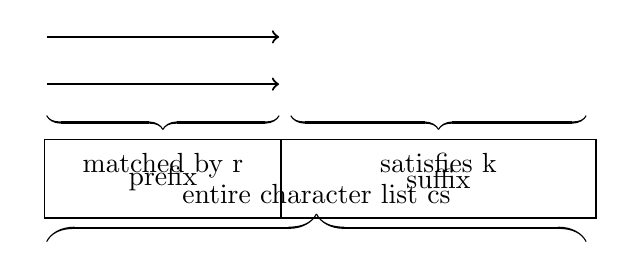
\begin{tikzpicture}
      \node[rectangle, draw=black, minimum height=1cm, minimum width=3cm] (L) {prefix};
      \node[right of=L, rectangle, draw=black, node distance=3.5cm, minimum width=4cm, minimum height=1cm] (R) {suffix};

      \node[above of=L, xshift=-1.6cm, yshift=-1.8cm] (TL) {};
      \node[above of=R, xshift=2cm, yshift=-1.8cm] (TR) {};

      \node[below of=L, xshift=-1.6cm, yshift=2.8cm] (IL) {};
      \node[below of=R, xshift=-1.9cm, yshift=2.8cm] (IR) {};
      \node[below of=L, xshift=-1.6cm, yshift=2.2cm] (IL2) {};
      \node[below of=R, xshift=-1.9cm, yshift=2.2cm] (IR2) {};

      \node[below of=L, xshift=-1.6cm, yshift=1.8cm] (UL) {};
      \node[below of=R, xshift=-1.9cm, yshift=1.8cm] (UR) {};
      \node[below of=L, xshift=1.5cm, yshift=1.8cm] (UL2) {};
      \node[below of=R, xshift=2cm, yshift=1.8cm] (UR2) {};
      \draw[-to, draw=black, thick] (IL) -- (IR);
      \draw[-to, draw=black, thick] (IL2) -- (IR2);
      \draw[thick, decorate, decoration={calligraphic brace, mirror, amplitude=5pt}] (UL) -- (UR)
        node[pos=0.5, below=10pt, black]{matched by \code{r}}
      ;
      \draw[thick, decorate, decoration={calligraphic brace, mirror, amplitude=5pt}] (UL2) -- (UR2)
        node[pos=0.5, below=10pt, black]{satisfies \code{k}}
      ;
      \draw[thick, decorate, decoration={calligraphic brace, amplitude=10pt}] (TL) -- (TR)
        node[pos=0.5, above=10pt, black]{entire character list \code{cs}}
      ;
    \end{tikzpicture}
  \end{center}

  \pause
  \vspace{-10pt}

  \lessonBox{\, Reasoning by specification or intuition is significantly more powerful
  than reasoning via stepping through code itself.}

\end{frame}
}

{
\renewcommand{\auxColor}{F48C6B}     % the color of note boxes and stuff
\renewcommand{\presentColor}{A827E4} % the primary color of the slide borders
\renewcommand{\bgColor}{eee6ff}      % the color of the background of the slide
\renewcommand{\darkBg}{8b98ad}
\renewcommand{\lambdaColor}{\auxColor}


\resetcolor

\customtitle{lecture12}

\begin{frame}[fragile]
  \frametitle{Lecture 12: Exceptions}

  We learned how to define \term{exceptions}, which are constructors of the
  \term{extensible type} \code{exn}, which can have arbitrarily many constructors
  added to it during runtime.

  \pause
  \vspace{\fill}

  \begin{codeblock}
    datatype exn = Match | Bind | Div | Fail of string | ...
  \end{codeblock}

  \pause
  \vspace{\fill}

  We saw how we could use exceptions as escape hatches during exceptional
  cases for functions, as well as ways to jump to \term{handlers} that
  can then continue on with the program.
\end{frame}

\begin{frame}[fragile]
  \frametitle{Lecture 12: Exceptions}

  This manifested in \term{exception-handling style}, which resembles
  CPS, but replaces a failure continuation with exceptions.

  \pause
  \vspace{\fill}

  \begin{codeblock}
    exception NotFound

    fun searchEHS p Empty = raise NotFound
      | searchEHS p (Node (L, x, R)) =
          if p x then
            x
          else
            (searchEHS p L) handle NotFound => searchEHS p R
  \end{codeblock}

  \pause
  \vspace{\fill}

  \lessonBox{\, It's OK to take quick, less-maintainable shortcuts, so long
  as you are judicious with their usage. Put simply, there's an \term{exception}
  to every rule.}

\end{frame}
}

{
\renewcommand{\auxColor}{03009A}     % the color of note boxes and stuff
\renewcommand{\presentColor}{0066FF} % the primary color of the slide borders
\renewcommand{\bgColor}{d8eff2}      % the color of the background of the slide
\renewcommand{\darkBg}{8b98ad}
\renewcommand{\lambdaColor}{\auxColor}

\resetcolor

\customtitle{lecture11}

\begin{frame}[fragile]
  \frametitle{Lecture 11: Continuation-Passing Style}

  We derive \term{continuation-passing style} by just considering what
  happens when we pass the result of a recursive call forward via piping
  into a lambda. So we might translate it as:


  \pause
  \begin{center}
  \begin{minipage}{0.45\textwidth}
    \raggedright

    First we replace all recursive calls with a placeholder variable.

    \vspace{10pt}

    Then we obtain the placeholder variables via just making recursive calls,
    and piping into an explicit lambda.

    \vspace{10pt}

    Observe that this is just extensionally equivalent to our original
    \code{treesum} function.
  \end{minipage}
  \begin{minipage}{0.5\textwidth}
    {\small
    \begin{codeblock}
      fun treesum Empty = 0
        | treesum (Node (L, x, R)) =
            treesum L + x + treesum R
    \end{codeblock}
    }
    {\small
    \begin{codeblock}
      fun treesum Empty = 0
        | treesum (Node (L, x, R)) =
            `resL` + x + `resR`
    \end{codeblock}
    }
    {\small
    \begin{codeblock}
      fun treesum Empty = 0
        | treesum (Node (L, x, R)) =
            `treesum L |> (fn resL =>`
            `treesum R |> (fn resR =>`
            resL + x + resR`))`
    \end{codeblock}
    }
  \end{minipage}
  \end{center}

\end{frame}

\begin{frame}[fragile]
  \frametitle{Lecture 11: Continuation-Passing Style}

  \begin{center}
  \begin{minipage}{0.45\textwidth}
    \raggedright
    This is not yet CPS, but what happens if we, instead of piping into a lambda, pass the lambda
    into the function itself?

    \vspace{10pt}

    Now, we derive CPS from very simple ideas! All we need to do is to make our recursive
    calls explicit.

    \vspace{10pt}

    \lessonBox{\, Complicated things can be made simple once you have an algorithm for it.}
  \end{minipage}
  \begin{minipage}{0.54\textwidth}
    {\small
    \begin{codeblock}
      fun treesumCPS Empty `k` = 0
        | treesumCPS (Node (L, x, R)) `k` =
            treesumCPS L & & (fn resL =>
            treesumCPS R & & (fn resR =>
            resL + x + resR))
    \end{codeblock}

    \begin{codeblock}
      fun treesumCPS Empty k = 0 `|> k`
        | treesumCPS (Node (L, x, R)) k =
            treesumCPS L (fn resL =>
            treesumCPS R (fn resR =>
            resL + x + resR `|> k`))
    \end{codeblock}
    }
  \end{minipage}
  \end{center}

\end{frame}
}

{
\renewcommand{\auxColor}{25a2db}     % the color of note boxes and stuff
\renewcommand{\presentColor}{FF68DE} % the primary color of the slide borders
\renewcommand{\bgColor}{e6fcff}      % the color of the background of the slide
\renewcommand{\darkBg}{8b98ad}
\renewcommand{\lambdaColor}{\auxColor}

\resetcolor

\customtitle{lecture10}

\begin{frame}[fragile]
  \frametitle{Lecture 10: Combinators and Staging}

  As a precursor to our eventual knowledge of streams and laziness, we
  found that we could control the evaluation of SML code via being particular
  about where it appeared relative to a given function's arguments.


  \pause
  \vspace{\fill}

  So that this function:
  \begin{codeblock}
    fun foo x y =
      horrible_computation x + y
  \end{codeblock}

  can instead be staged as such:
  \pause
  \begin{codeblock}
    fun foo x & & =
      `let`
        `val res = horrible_computation x`
      `in`
        `fn y =>` `res` + y
      `end`
  \end{codeblock}
\end{frame}

\begin{frame}[fragile]
  \frametitle{Lecture 10: Combinators and Staging}

  We then learned about piping operators like
  \code{|>}, which represent an ultimate form of
  higher-order programming, that lets us manipulate the format of
  any code to our liking.

  \pause
  \vspace{\fill}

  {\small
  \begin{codeblock}
    remove (wait 2 (insert trayOfMozzarellaSticks (heat oven 400)))
  \end{codeblock}
  }

  \pause
  \vspace{\fill}

  \begin{codeblock}
    heat oven 400
    |> insert trayOfMozzarellaSticks
    |> wait 2
    |> remove
  \end{codeblock}

  \pause
  \vspace{\fill}

  \lessonBox{\, Pretty privilege is OK when it applies to code.}
\end{frame}
}

{

\renewcommand{\auxColor}{b39c09}     % the color of note boxes and stuff
\renewcommand{\presentColor}{32A2A5} % the primary color of the slide borders
\renewcommand{\bgColor}{d1eff0}      % the color of the background of the slide
\renewcommand{\darkBg}{8b98ad}
\renewcommand{\lambdaColor}{\auxColor}


\resetcolor

\customtitle{lecture9}

\begin{frame}[fragile]
  \frametitle{Lecture 9: Higher-Order Functions}

  Here, we learned about \term{currying}, which is simply
  a function which takes in "multiple arguments", by returning a
  function which takes the rest of the arguments.

  \pause
  \vspace{\fill}

  \begin{codeblock}
    (* add : int * int -> int *)
    fun add (x, y) = x + y

    (* addC : int -> int -> int *)
    val addC = fn x => fn y =>
    (* syntactic sugar! *)
    fun addC x y = x + y
  \end{codeblock}

  \pause
  \vspace{\fill}

  We saw that, just by adjusting our perspective, something as
  simple as functions being able to return something of function
  type would have a massive influence on our style of programming.
\end{frame}

\begin{frame}[fragile]
  \frametitle{Lecture 9: Higher-Order Functions}

  We also saw the role that higher-order functions have
  in terms of being able to capture the very design
  patterns of our code.

  \pause
  \vspace{\fill}

  So then, seen in this light, functions like \code{sum} and
  \code{concat} have the same "DNA" -- the information content
  of their code follows the same pattern.

  \pause
  \vspace{\fill}

  \begin{codeblock}
    fun sum [] = 0
      | sum (x::xs) = x + sum xs

    fun concat [] = ""
      | concat (x::xs) = x ^ concat xs
  \end{codeblock}
\end{frame}

\begin{frame}[fragile]
  \frametitle{Lecture 9: Higher-Order Functions}

  Higher-order functions are an essential tool in functional programming that
  are pivotal to many of the things we studied later.

  \pause
  \vspace{\fill}

  HOFs ultimately ended up opening the first conceptual door to much greater
  things, such as \code{match}, such as CPS, and such as many of the functions
  we could write on streams and sequences. Through it, we see that great things
  come out of simply thinking of functions as values.

  \pause
  \vspace{\fill}

  \lessonBox{\, Writing code is good. Writing code which writes code is better.}

\end{frame}

}


{
\renewcommand{\auxColor}{039c1a}     % the color of note boxes and stuff
\renewcommand{\presentColor}{E45535} % the primary color of the slide borders
\renewcommand{\bgColor}{e3f3ff}      % the color of the background of the slide
\renewcommand{\darkBg}{8b98ad}
\renewcommand{\lambdaColor}{\auxColor}

\resetcolor

\customtitle{lecture8}

\begin{frame}[fragile]
  \frametitle{Lecture 8: Polymorphism}

  Before we could learn about higher-order functions, however, we needed to
  have a more expressive type system, to talk about functions of potentially
  arbitrary type.

  \pause
  \vspace{\fill}

  Staging\footnote{haha} that lecture was the idea of \term{polymorphism},
  which expanded our vocabulary of types to include \term{type variables}
  like \code{'a}, \code{'b}, and \code{'c}, which allowed us to talk about
  types which may be instantiated at more specific type.

  \pause
  \vspace{\fill}

  This ended up giving us a vast amount of flexibility, by allowing us to
  write generic functions that can be used a type-safe way, by merely
  varying the type with the context of its use.

  \pause
  \vspace{\fill}

  We also saw that we could execute \term{typing traces} by collecting
  constraints on arguments to functions, which are given an initial,
  unrestricted type variable, and then coming up with its \term{most general type}.
\end{frame}

\begin{frame}[fragile]
  \frametitle{Lecture 8: Polymorphism}

  \begin{center}
    \makebox[0.8\textwidth][c]{
      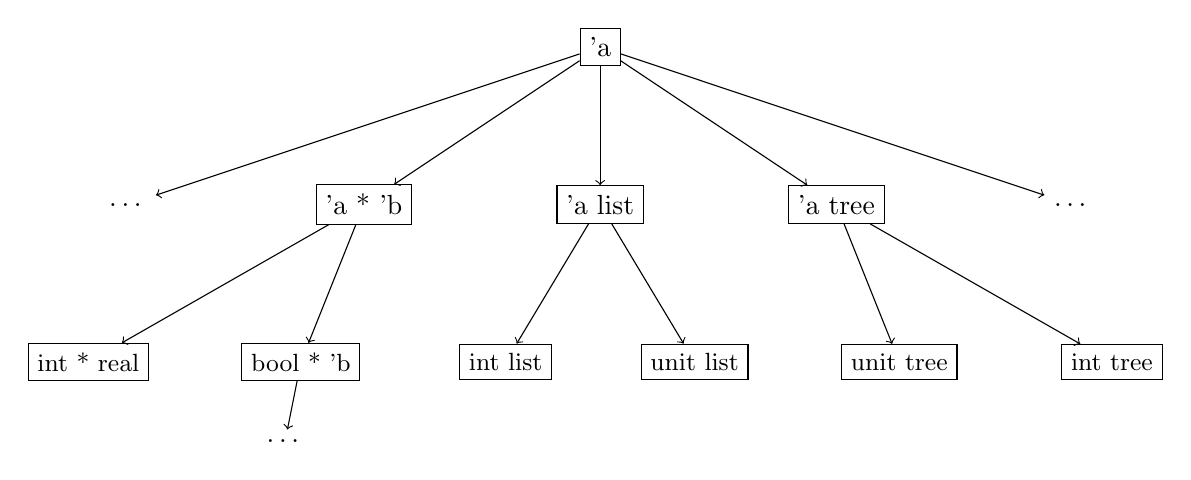
\begin{tikzpicture}
        \node[shape=rectangle,draw=black] (L1) at (-4.5,0) {\small \code{int * real}};

        \node[] (E2) at (-2,-1) {\textellipsis};
        \node[shape=rectangle,draw=black] (L2) at (-1.8,0) {\small \code{bool * 'b}};

        \node[shape=rectangle,draw=black] (L3) at (0.8,0) {\small \code{int list}};

        \node[shape=rectangle,draw=black] (L4) at (3.2,0) {\small \code{unit list}};

        \node[shape=rectangle,draw=black] (L5) at (5.8,0) {\small \code{unit tree}};

        \node[shape=rectangle,draw=black] (L6) at (8.5,0) {\small \code{int tree}};

        \node[] (EL) at (-4,2) {\textellipsis};
        \node[shape=rectangle,draw=black] (M1) at (-1,2) {\code{'a * 'b}};
        \node[shape=rectangle,draw=black] (M2) at (2,2) {\code{'a list}};
        \node[shape=rectangle,draw=black] (M3) at (5,2) {\code{'a tree}};
        \node[] (ER) at (8,2) {\textellipsis};

        \node[shape=rectangle,draw=black] (T) at (2,4) {\code{'a}};

        \draw[<-] (E2) -- (L2);

        \draw[<-] (L1) -- (M1);
        \draw[<-] (L2) -- (M1);
        \draw[<-] (L3) -- (M2);
        \draw[<-] (L4) -- (M2);
        \draw[<-] (L5) -- (M3);
        \draw[<-] (L6) -- (M3);

        \draw[<-] (EL) -- (T);
        \draw[<-] (M1) -- (T);
        \draw[<-] (M2) -- (T);
        \draw[<-] (M3) -- (T);
        \draw[<-] (ER) -- (T);
    \end{tikzpicture}
    }
    \end{center}

  \pause
  \lessonBox{\, More advanced type structure leads to concrete benefits in code. In
  other words, \term{types guide structure}.}

\end{frame}
}

{
\renewcommand{\auxColor}{5725E4}     % the color of note boxes and stuff
\renewcommand{\presentColor}{FABC60} % the primary color of the slide borders
\renewcommand{\bgColor}{fff8ed}      % the color of the background of the slide
\renewcommand{\darkBg}{8b98ad}
\renewcommand{\lambdaColor}{\auxColor}

\resetcolor

\newcommand{\mygreen}[0]{%
\color{green!55!black}
}

\customtitle{lecture7}

\begin{frame}[fragile]
  \frametitle{Lecture 7: Sorting and Parallelism}

  Back at this point in the course, we were more concerned with the
  mathematics and formal parts of analyzing our code.

  \pause
  \vspace{\fill}

  We learned about the \term{tree method}, which allows us to solve
  recurrences that make more than one "recursive call" per level. We
  think of the tree method as simply inducing a "call tree" which
  denotes all of the calls being made by the recursive function,
  annotated with the size of the input and the nonrecursive work at
  each node.

  \pause
  \vspace{\fill}

  This ended up being a pivotal tool in analyzing such recursive
  functions, which came out of simply thinking about how we would sum the
  nonrecursive work at each level of the call tree, and then applying some
  simple mathematical facts.
\end{frame}

\begin{frame}[fragile]
  \frametitle{Lecture 7: Sorting and Parallelism}

  For instance, we might draw a call tree labeled with the size of
  each node for the recurrence where eachh $W(n)$ term expands to
  contain $2W(n)$:

  \pause
  \vspace{\fill}

  \makebox[\textwidth][c]{
    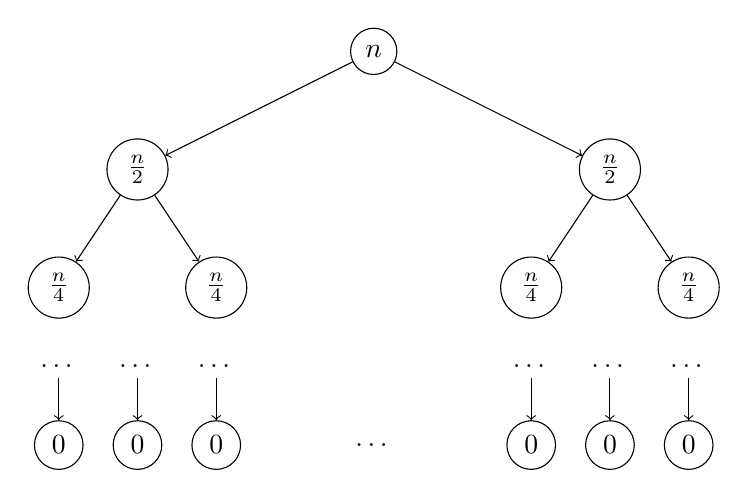
\begin{tikzpicture}
      \node[shape=circle,draw=black] (T) at (2,4) { $n$} ;

      \node[shape=circle,draw=black] (M1) at (-1,2.5) { $\frac{n}{2}$};
      \node[shape=circle,draw=black] (M2) at (5,2.5) { $\frac{n}{2}$};

      \node[shape=circle,draw=black] (L1) at (-2,1) { $\frac{n}{4}$};
      \node[shape=circle,draw=black] (L2) at (0,1) { $\frac{n}{4}$};

      \node[shape=circle,draw=black] (L3) at (4,1) { $\frac{n}{4}$};
      \node[shape=circle,draw=black] (L4) at (6,1) { $\frac{n}{4}$};

      \node[shape=circle,draw=black] (LL1) at (-2,-1) { $0$};
      \node[shape=circle,draw=black] (LL2) at (-1,-1) { $0$};
      \node[shape=circle,draw=black] (LL3) at (0,-1) { $0$};

      \node[shape=circle,draw=black] (LL4) at (4,-1) { $0$};
      \node[shape=circle,draw=black] (LL5) at (5,-1) { $0$};
      \node[shape=circle,draw=black] (LL6) at (6,-1) { $0$};

      \node[] (LLM) at (2,-1) { \textellipsis};

      \node [above of=LL1] (ULL1) {\textellipsis};
      \node [above of=LL2] (ULL2) {\textellipsis};
      \node [above of=LL3] (ULL3) {\textellipsis};
      \node [above of=LL4] (ULL4) {\textellipsis};
      \node [above of=LL5] (ULL5) {\textellipsis};
      \node [above of=LL6] (ULL6) {\textellipsis};

      \draw[->] (T) -- (M1);
      \draw[->] (T) -- (M2);

      \draw[->] (M1) -- (L1);
      \draw[->] (M1) -- (L2);
      \draw[->] (M2) -- (L3);
      \draw[->] (M2) -- (L4);

      \draw[->] (ULL1) -- (LL1);
      \draw[->] (ULL2) -- (LL2);
      \draw[->] (ULL3) -- (LL3);
      \draw[->] (ULL4) -- (LL4);
      \draw[->] (ULL5) -- (LL5);
      \draw[->] (ULL6) -- (LL6);
  \end{tikzpicture}
  }
\end{frame}

\begin{frame}[fragile]
  \frametitle{Lecture 7: Sorting and Parallelism}

  Or, for a specific example, we might also do this for the
  \code{inord} function:

  \vspace{-15pt}

  $$W_{\code{inord}}({\color{green!55!black} n}) = {\color{auxColor} c_1 + W_{\code{@}}(\frac{n}{2})} + {\color{red} 2 \cdot W_{\code{inord}}(\frac{n}{2})}$$

  \pause
  \makebox[\textwidth][c]{
    \begin{tikzpicture}
      \node[shape=rectangle,draw=black] (T) at (2,4) { ${\mygreen n} \, \vert \,  {\color{auxColor} c_2 \cdot \frac{n}{2}}$ } ;

      \node[shape=rectangle,draw=black] (M1) at (-1,2.5) { ${ \mygreen \frac{n}{2}} \, \vert \, {\color{auxColor} c_2 \cdot \frac{n}{4}}$};
      \node[shape=rectangle,draw=black] (M2) at (5, 2.5) { ${ \mygreen \frac{n}{2}} \, \vert \, {\color{auxColor} c_2 \cdot \frac{n}{4}}$};

      \node[shape=rectangle,draw=black] (L1) at (-2,1) { ${ \mygreen \frac{n}{4}} \, \vert \, {\color{auxColor} c_2 \cdot \frac{n}{8}}$};
      \node[shape=rectangle,draw=black] (L2) at (0,1) { ${ \mygreen \frac{n}{4}} \, \vert \, {\color{auxColor} c_2 \cdot \frac{n}{8}}$};

      \node[shape=rectangle,draw=black] (L3) at (4,1) { ${ \mygreen \frac{n}{4}} \, \vert \, {\color{auxColor} c_2 \cdot \frac{n}{8}}$};
      \node[shape=rectangle,draw=black] (L4) at (6.5,1) { ${ \mygreen \frac{n}{4}} \, \vert \, {\color{auxColor} c_2 \cdot \frac{n}{8}}$};

      \node[shape=rectangle,draw=black] (LL1) at (-3,-1) { ${\mygreen 0} \, \vert \, {\color{auxColor} c_0}$};
      \node[shape=rectangle,draw=black] (LL2) at (-1.5,-1) { ${\mygreen 0} \, \vert \, {\color{auxColor} c_0}$};
      \node[shape=rectangle,draw=black] (LL3) at (0, -1) { ${\mygreen 0} \, \vert \, {\color{auxColor} c_0}$};

      \node[shape=rectangle,draw=black] (LL4) at (4,-1) { ${\mygreen 0} \, \vert \, {\color{auxColor} c_0}$};
      \node[shape=rectangle,draw=black] (LL5) at (5.5,-1) { ${\mygreen 0} \, \vert \, {\color{auxColor} c_0}$};
      \node[shape=rectangle,draw=black] (LL6) at (7, -1) { ${\mygreen 0} \, \vert \, {\color{auxColor} c_0}$};

      %\node[] (D1) at (-5, 4) { $= 2^0 \cdot {\color{auxColor} c_2 \cdot \frac{n}{2}} = c_1 \cdot \frac{n}{2}$ };
      %\node[] (D2) at (-5, 1) { $= 2^1 \cdot {\color{auxColor} c_2 \cdot \frac{n}{2}} = c_1 \cdot \frac{n}{2}$ };
      %\node[] (D3) at (-5, -1) { $= 2^2 \cdot {\color{auxColor} c_2 \cdot \frac{n}{2}} = c_1 \cdot \frac{n}{2}$ };

      \node[] (S1) at (9.5, 4) { $= 2^0 \cdot {\color{auxColor} c_2 \cdot \frac{n}{2}} = c_2 \cdot \frac{n}{2}$ };
      \node[] (S2) at (9.5, 2.5) { $= 2^1 \cdot {\color{auxColor} c_2 \cdot \frac{n}{4}} = c_2 \cdot \frac{n}{2}$ };
      \node[] (S3) at (9.5, 1) { $= 2^2 \cdot {\color{auxColor} c_2 \cdot \frac{n}{8}} = c_2 \cdot \frac{n}{2}$ };
      \node[] (S4) at (9.5, -1) { $= \frac{n}{2} \cdot {\color{auxColor} c_0} = c_0 \cdot \frac{n}{2}$ };

      \node[] (LLM) at (2,-1) { \textellipsis};

      \node [above of=LL1] (ULL1) {\textellipsis};
      \node [above of=LL2] (ULL2) {\textellipsis};
      \node [above of=LL3] (ULL3) {\textellipsis};
      \node [above of=LL4] (ULL4) {\textellipsis};
      \node [above of=LL5] (ULL5) {\textellipsis};
      \node [above of=LL6] (ULL6) {\textellipsis};

      \draw[->] (T) -- (M1);
      \draw[->] (T) -- (M2);

      \draw[->] (M1) -- (L1);
      \draw[->] (M1) -- (L2);
      \draw[->] (M2) -- (L3);
      \draw[->] (M2) -- (L4);

      \draw[->] (ULL1) -- (LL1);
      \draw[->] (ULL2) -- (LL2);
      \draw[->] (ULL3) -- (LL3);
      \draw[->] (ULL4) -- (LL4);
      \draw[->] (ULL5) -- (LL5);
      \draw[->] (ULL6) -- (LL6);
  \end{tikzpicture}
  }
\end{frame}

\begin{frame}[fragile]
  \frametitle{Lecture 7: Sorting and Parallelism}

  We then learned about \code{span}, the idea of the \textit{parallel cost}
  of our code, where we assume that we have an infinite number of processors.

  \pause
  \vspace{\fill}

  Due to intrinsic \term{data dependencies} in code, having infinitely
  many processors doesn't necessarily solve all our problems, but it
  means that we can achieve a smaller cost bound for certain kinds of problems.
  This is because we take the \textbf{max} over certain parallelizable
  operations, rather than sequentially taking the \textbf{sum}.

  \pause
  \vspace{\fill}

  We saw this in a use case for \term{merge sort}, where we could achieve a
  $O(\log n)$ span via parallelism, which also admitted an extremely
  simple implementation.
\end{frame}

\begin{frame}[fragile]
  \frametitle{Lecture 7: Sorting and Parallelism}

  {\tiny
  \begin{codeblock}
    fun split ([] : int list) : int list * int list = []
      | split [x] = [x]
      | split (x::y::xs) =
          let
            val (A, B) = split xs
          in
            (x::A, y::B)
          end

    fun merge ([] : int list, R : int list) : int list = R
      | merge (L, []) = L
      | merge (x::xs, y::ys) =
          if x < y then
            x :: merge (xs, y::ys)
          else
            y :: merge (x::xs, ys)

    fun msort ([] : int list) : int list = []
      | msort [x] = [x]
      | msort L =
          let
            val (A, B) = split L
          in
            merge (msort A, msort B)
          end
  \end{codeblock}
  }

  \pause
  \lessonBox{\, Complicated things admit a simple recursive implementation,
  which also gives way to a simple recursive mathematical analysis.}
\end{frame}

}

{
\renewcommand{\auxColor}{FF4F4F}     % the color of note boxes and stuff
\renewcommand{\presentColor}{FFAB73} % the primary color of the slide borders
\renewcommand{\bgColor}{fff3e6}      % the color of the background of the slide
\renewcommand{\darkBg}{8b98ad}
\renewcommand{\lambdaColor}{\auxColor}

\resetcolor

\customtitle{lecture6}

\begin{frame}[fragile]
  \frametitle{Lecture 6: Asymptotic Analysis}

  But before we could learn about parallel complexity, we learned about
  generally ascertaining the mathematical run-time of some function.

  \pause
  \vspace{\fill}

  We learned how to do this by writing a \term{recurrence} for the
  abstract units of cost incurred by a given recursive function. We
  generally had to write our recurrences in terms of some notion of
  size of the input. For instance, the \code{treesum} function:

  \begin{codeblock}
    fun treesum Empty = 0
      | treesum (Node (L, x, R)) = treesum L + x + treesum R
  \end{codeblock}
\end{frame}

\begin{frame}[fragile]
  \frametitle{Lecture 6: Asymptotic Analysis}

  This ends up producing the recurrence, in terms of the number of nodes of
  the tree $n$,

  $$W_{\code{treesum}}(0) = c_0$$
  $$W_{\code{treesum}}(n) = W_{\code{treesum}}(n_l) + c_1 + W_{\code{treesum}}(n_r)$$

  where $n_l$ and $n_r$ are the number of nodes in the left and right subtrees,
  respectively.

  \pause
  \vspace{\fill}

  \lessonBox{\, Mathematical analysis can make even the most convoluted of things
  understandable.}
\end{frame}
}

{
\renewcommand{\auxColor}{6e3b0d}     % the color of note boxes and stuff
\renewcommand{\presentColor}{FFABE1} % the primary color of the slide borders
\renewcommand{\bgColor}{fef7ff}      % the color of the background of the slide
\renewcommand{\darkBg}{8b98ad}
\renewcommand{\lambdaColor}{\auxColor}

\resetcolor

\customtitle{lecture5}

\begin{frame}[fragile]
  \frametitle{Lecture 5: Trees}

  Here, we learned about \term{trees} and other custom datatype declarations,
  called \term{algebraic datatypes}.

  \pause
  \vspace{\fill}

  We saw that structural induction could be carried out on any arbitrary
  recursive datatype, even including things which did not look like lists or
  induction!

  \pause
  \vspace{\fill}

  Our previous view of induction was a narrow one, but we would later
  learn that induction is more of a spectrum, ranging over a wide variety
  of types and data structures.
\end{frame}

\begin{frame}[fragile]
  \frametitle{Lecture 5: Trees}

  In particular, we found that when inducting on a non-traditional structure,
  like a tree, the \textbf{proof follows the code}. If a constructor has two
  recursive sub-components (such as \code{Node}), then the proof gets
  two inductive hypotheses.

  \pause
  \vspace{\fill}

  Writing code is like writing a proof. Decouple the two in your mind when
  writing code that is meant to be correct -- the process of writing the
  code should be akin to proving that it is correct.

  \pause
  \vspace{\fill}

  \lessonBox{\, An impoverished view of programming fits problems to a small
  set of base types. A rich view of programming fits types to problems.}
\end{frame}
}

{
\renewcommand{\auxColor}{008a25}     % the color of note boxes and stuff
\renewcommand{\presentColor}{1FAB89} % the primary color of the slide borders
\renewcommand{\bgColor}{f5fff5}      % the color of the background of the slide
\renewcommand{\darkBg}{8b98ad}
\renewcommand{\lambdaColor}{\auxColor}


\resetcolor

\customtitle{lecture4}

\begin{frame}[fragile]
  \frametitle{Lecture 4: Structural Induction and Tail Recursion}

  \term{Structural induction} was taught as an upgrade of normal induction,
  where the structure of a list could be observed as similar to the structure of
  the natural numbers.

  \pause
  \vspace{\fill}

  Just like how we had $n$ and $n + 1$, we drew an analogy to the
  structure of a list as \code{xs} and \code{x::xs}.

  \pause
  \vspace{\fill}

  The idea of \term{parse, don't validate} was introduced, which consists
  of \textbf{expressing your information through types} when possible,
  rather than flattening it down to something as simple and without depth
  as a boolean. We saw this in the translation of the function \code{take}:
\end{frame}

\begin{frame}[fragile]
  \frametitle{Lecture 4: Structural Induction and Tail Recursion}

  {\small
  \begin{codeblock}
    fun take (n : int, L : int list) : int list =
      if isEmpty L orelse n = 0 then
        []
      else
        let
          val x = hd L
          val xs = tl L
        in
          x :: take (n - 1, xs)
        end
  \end{codeblock}

  \begin{codeblock}
    fun take (n : int, L : int list) : int list =
      case (n, L) of
        (0, _)     => []
      | (_, [])    => []
      | (_, x::xs) => x :: take (n - 1, xs)
  \end{codeblock}
  }
\end{frame}

\begin{frame}[fragile]
  \frametitle{Lecture 4: Structural Induction and Tail Recursion}

  Here, we also started learning about the importance of \term{totality}
  in proofs. We learned about the necessity of totality as a tool to
  get at valuability, so that we could step through code that relied
  on some form of eager evaluation.

  \pause
  \vspace{\fill}

  \begin{center}
    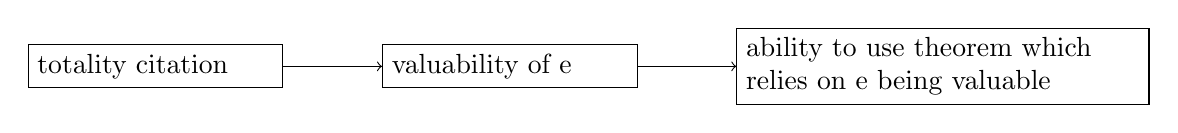
\begin{tikzpicture}
      \node[shape=rectangle,draw=black, text width=3cm] (M1) at (-3,2) {totality citation};
      \node[shape=rectangle,draw=black, text width=3cm] (M2) at (1.5,2) {valuability of \code{e}};
      \node[shape=rectangle,draw=black, text width=5cm] (M3) at (7,2) {ability to use theorem which \\ relies on \code{e} being valuable};

      \draw[->] (M1) -- (M2);
      \draw[->] (M2) -- (M3);
    \end{tikzpicture}
  \end{center}

  \pause
  \vspace{\fill}

  \lessonBox{\, \textbf{Parse, don't validate!} Express your data through types
  when you can.}

\end{frame}
}

{
\renewcommand{\auxColor}{0f8a73}     % the color of note boxes and stuff
\renewcommand{\presentColor}{002B5B} % the primary color of the slide borders
\renewcommand{\bgColor}{a6c4e3}      % the color of the background of the slide
\renewcommand{\darkBg}{8b98ad}
\renewcommand{\lambdaColor}{\auxColor}

\resetcolor

\customtitle{lecture3}

\begin{frame}[fragile]
  \frametitle{Lecture 3: Induction and Recursion}

  But before we could get to the idea of structural induction, we first
  had to talk about normal \term{induction} on the natural numbers.

  \pause
  \vspace{\fill}

  We see now that induction on the natural numbers can be thought of as just
  an instance of structural induction on the following datatype:
  \begin{codeblock}
    datatype nat = Zero | Succ of nat
  \end{codeblock}

  \pause
  \vspace{\fill}

  When it comes down to it, induction should be hard-wired into your brain.
  \textbf{Base case, induction hypothesis, inductive step, repeat.}

  \pause
  \vspace{\fill}

  We also learned about the \term{"recursive leap of faith"} method for writing a
  recursive function, which simply requires a leap of faith that your
  function works, to write a function which does the right thing.

  \pause
  \vspace{\fill}

  \lessonBox{\, We call the method of solving an infinite amount of problems in
  finite space, "induction", or "recursion", and they are the same thing.}

\end{frame}
}

{
\renewcommand{\auxColor}{009999}     % the color of note boxes and stuff
\renewcommand{\presentColor}{50009F} % the primary color of the slide borders
\renewcommand{\bgColor}{d3cade}      % the color of the background of the slide
\renewcommand{\darkBg}{d4cedb}
\renewcommand{\lambdaColor}{\auxColor}

\resetcolor

\customtitle{lecture2}

\begin{frame}[fragile]
  \frametitle{Lecture 2: Equivalence, Binding, and Scope}

  Back during this lecture, we were still getting a hold of the basics of
  SML!

  \pause
  \vspace{\fill}

  We learned about \term{extensional equivalence}, which turned out to be a
  pivotal notion in our understanding of programs, and of our understanding of
  how to write \textit{correct} programs.

  \pause
  \vspace{\fill}

  To facilitate this idea, we introduced the concept of \term{binding}, which
  differs from other programming languages which have \term{assignment}, in that
  the value of a variable never changes, when it is bound. That variable can only
  be \term{shadowed} with a different, unrelated binding that shares the same
  name.

  \pause
  \vspace{\fill}

  This ultimately introduced the idea of \term{immutability}, or simply not
  allowing values to mutate wildly in a single context. This means that code
  reads the same as math -- values are values.

  \pause
  \vspace{\fill}

  \lessonBox{\, Binding is not assignment! We can gain many benefits from simply
  adopting an immutable style.}

\end{frame}
}

{
\renewcommand{\auxColor}{2791e3}
\renewcommand{\presentColor}{2e2e2e} % the primary color of the slide borders
\renewcommand{\bgColor}{d6d6d6}      % the color of the background of the slide
\renewcommand{\darkBg}{8b98ad}
\renewcommand{\lambdaColor}{\auxColor}

\resetcolor

\customtitle{lecture1}

\begin{frame}[fragile]
  \frametitle{Lecture 1: Prologue}

  And then, at the start of everything, we had our first lecture.

  \pause
  \vspace{\fill}

  This lecture introduced the Standard ML language, it introduced the
  idea of having a strong type discipline, and it made a few promises.

  \pause
  \vspace{\fill}

  On the very first day, we set out with an idea of what we wanted
  programming to be. We also laid out our \term{Three Theses}, which
  have appeared so far throughout the slides, and throughout the
  course.

  \pause
  \vspace{\fill}

  \lessonBox{\, Functional programming is an improvement on our ability
  to program. It is a refinement on our ability to communicate, as
  programmers.}

  \pause
  \vspace{\fill}

  How have we kept on on those promises, and foreshadowings?
\end{frame}
}

\sectionSlide{2}{Course Themes}

\begin{frame}[fragile]
  \frametitle{What is Programming?}

  On the first day, I posed this question to you. What is programming? What is
  good programming? What should good programming be?

  \pause
  \vspace{\fill}

  Let's revisit those answers.

  \pause
  \vspace{\fill}

  Programming should be:
  \pause
  \begin{itemize}
    \item descriptive
    \item modular
    \item maintainable
  \end{itemize}
\end{frame}

\begin{frame}[fragile]
  \frametitle{Programming Should Be: Descriptive}

  Programming should be \textbf{descriptive}.

  \pause
  \vspace{\fill}

  At this point in the course, we've seen many examples of this. Writing
  signatures that describe the interfaces of our code is one way of making
  our code more descriptive.

  \pause
  \vspace{\fill}

  Giving our code concrete, well-specified invariants that we can think of,
  when programming is another way of writing descriptive code.

  \pause
  \vspace{\fill}

  More generally, having powerful language constructs like
  higher-order functions, parametric polymorphism, and algebraic datatypes
  makes our programming incredibly expressive, and able to describe a wide
  array of problems.
\end{frame}

\begin{frame}[fragile]
  \frametitle{Programming Should Be: Modular}

  Programming should be \textbf{modular}.

  \pause
  \vspace{\fill}

  What better way to validate this claim than our discussion of literal
  modules? We saw that modules can be used to make composable software, or
  software that can be defined in terms of other, well-specified software
  components.

  \pause
  \vspace{\fill}

  If we had a library for \code{IntSet}, refactoring the internal implementation
  is incredibly easy, when we hide the details via opaque ascription. We
  saw that outside callers literally cannot depend on things which are hidden
  behind the interface, making for modular code.

  \pause
  \vspace{\fill}

  A strong typing discipline lends itself to modular code as well. Each expression
  and each variable has its own type, which gives it well-specified semantics and
  a well-specified way to interact with other parts of a modular codebase.
\end{frame}

\begin{frame}[fragile]
  \frametitle{Programming Should Be: Maintainable}

  Programming should be \textbf{maintainable}.

  \pause
  \vspace{\fill}

  More generally, the principle of extensional equivalence, or as I call it,
  the refactoring lemma, means we can \textbf{always} swap equivalent code
  for equivalent code. This is enormously powerful when it comes to refactoring
  and maintaining code.

  \pause
  \vspace{\fill}

  More generally, a strong typing discipline means that maintaining code is
  less likely to run into errors. You can't accidentally swap an expression
  of type \code{int} for one of type \code{int tree}, at least not easily.

  \pause
  \vspace{\fill}

  Functional code is not just nice to look at -- terser, more understandable
  code will ultimately lead to more maintainability. You cannot maintain
  code that you do not understand.
\end{frame}

\begin{frame}[fragile]
  \frametitle{Three Theses}

  What about the three theses that we learned?

  \pause
  \vspace{\fill}

  Those were:
  \pause
  \begin{itemize}
    \item \term{Recursive Problems, Recursive Solutions} \pause
    \item \term{Programmatic Thinking is Mathematical Thinking} \pause
    \item \term{Types Guide Structure}
  \end{itemize}
\end{frame}

\begin{frame}[fragile]
  \frametitle{Three Theses: Recursive Problems, Recursive Solutions}

  \term{Recursive Problems, Recursive Solutions} is about not letting recursion
  be the bogeyman.

  \pause
  \vspace{\fill}

  We've dealt with recursion all semester -- by this point, we're pros at it.
  Recursion is a technique that isn't something to be feared or excluded,
  it's a fundamental technique that is applicable in many scenarios.

  \pause
  \vspace{\fill}

  Through proper command of thinking with specifications and thinking with
  invariants, recursion becomes second nature. Ultimately, the recursive
  nature of linked lists and tree-like structures benefits a recursive
  approach.
\end{frame}

\begin{frame}[fragile]
  \frametitle{Three Theses: Programmatic Thinking is Mathematical Thinking}

  \term{Programmatic Thinking is Mathematical Thinking} is about the fact that
  computer scientists were mathematicians first.

  \pause
  \vspace{\fill}

  Before we can write any serious code, we have to be able to think about
  it in analytical code. Before we can write code which solves problems,
  we need to adopt a problem-solving mindset. It just so happens that
  math is the language of stating and solving problems.

  \pause
  \vspace{\fill}

  Work and span, induction, extensional equivalence, and adopting formal
  mathematical specifications are all different ways that math shows up in our
  code. Embrace it -- it can only make your ability to understand and
  solve problems better.
\end{frame}

\begin{frame}[fragile]
  \frametitle{Three Theses: Types Guide Structure}

  \term{Types Guide Structure} is about letting types dictate your thinking.

  \pause
  \vspace{\fill}

  Types are the language of programs, and the blueprints that software
  architectures are built upon. The exchange, construction, destruction,
  and interplay of data are all processes that are codified via
  types.

  \pause
  \vspace{\fill}

  We saw how powerful concepts like currying, HOFs, CPS, laziness, and
  polymorphism can come out of simply adjusting our type structure slightly.
  Seen in this way, we truly do let types guide the structure of our programs,
  and produce better code for it.
\end{frame}

\begin{frame}[fragile]
  \frametitle{Sayings}

  In addition to those, however, over the course of the semester I isolated
  some of the common sayings or idioms that tended to crop up during
  each lesson.

  \pause
  \vspace{\fill}

  Some lessons are planned. Others must be discovered. These ones are the
  latter.

  \pause
  \vspace{\fill}

  \begin{itemize}
    \item Be Clever by Being Dumb \pause
    \item Self-Defence Against Yourself \pause
    \item We Are in the Business of Writing Correct Code \pause
    \item Do It Better
  \end{itemize}
\end{frame}

\begin{frame}[fragile]
  \frametitle{Sayings: Be Clever by Being Dumb}

  I don't think I necessarily ever said this one out loud, but I was
  thinking it.

  \pause
  \vspace{\fill}

  Some people think I like functional programming because I am smart. These
  people are incredibly wrong. I like functional programming because I am
  extremely prone to stupid mistakes, and without good code to support me,
  I would never get anything done.

  \pause
  \vspace{\fill}

  At this point in the course, we've discussed the type-checker, and all
  the ways that it serves as both our best friend and our worst enemy. I
  am squarely in the "best friend" camp, because without the typechecker
  at my side 90\% of the code I write would be nonsense.
\end{frame}

\begin{frame}[fragile]
  \frametitle{Sayings: Be Clever by Being Dumb}

  Learning how to program (or computer science in general) is a massive
  rush of learning new skills and techniques, fancy names, and cool buzzwords
  that seem to clue you in on a brand new world.

  \pause
  \vspace{\fill}

  In my experience, learning how to program well has entailed learning how to
  cut back on that instinctive desire to do things in a "cool" or "clever" way.

  \pause
  \vspace{\fill}

  Cool is cool. Clever is clever. But clever is not maintainable. Nobody
  wants to read your "clever" code which requires five different assumptions
  to understand.

  \pause
  \vspace{\fill}

  Write code which speaks for itself. Write code that is simple and expressive,
  and gets the job done in the least confusing way possible. To me, that is
  what functional programming stands for.
\end{frame}

\begin{frame}[fragile]
  \frametitle{Sayings: Self-Defence Against Yourself}

  This has been a class on learning how to program well.

  \pause
  \vspace{\fill}

  The main way that we can learn how to program well is to learn how to
  live with ourselves, as programmers. We are often our own worst enemies,
  writing code which is inunderstandable merely hours later, or leaving
  footguns in our code that future versions of ourself have to deal with.

  \pause
  \vspace{\fill}

  To that end, the first step in learning to program well is to learn how to
  defend yourself against yourself. Writing safe, correct code requires that
  you be able to prevent yourself from making mistakes, because every programmer
  makes mistakes.

  \pause
  \vspace{\fill}

  So let's prevent type errors, let's prevent dynamic errors instead of static ones,
  let's prevent ourselves from having to write messy code which we will have to
  deal with later. Making mistakes is OK, let's just minimize the chances.
\end{frame}

\begin{frame}[fragile]
  \frametitle{Sayings: We Are in the Business of Writing Correct Code}

  Something I \textit{have} said multiple times is that we are not in
  the business of writing code, we are in the business of writing
  \textit{correct} code.

  \pause
  \vspace{\fill}

  Some people are in the business of writing code. They look for code
  output and productivity measured in terms of silly metrics that have
  nothing to do with actual impact.

  \pause
  \vspace{\fill}

  That's cool, but we're here to write correct code. We're here to do
  things right. Because nobody wants software which doesn't work. We
  want to make sure that our code is right, so we have things like
  extensional equivalence, reasoning via specification, and type safety
  to guide us towards that.
\end{frame}

\begin{frame}[fragile]
  \frametitle{Sayings: Do It Better}

  Do it, but do it better. Or, alternatively, we can do better.

  \pause
  \vspace{\fill}

  Self-improvement is a process of first being open to improvement.
  Knowing how to program is good, but a theme throughout this course has
  been learning the numerous ways that we can improve our ability to
  program.

  \pause
  \vspace{\fill}

  Knowing how to do something is cool, but you need to always be on the
  lookout for how to improve, if you want to really be good at something.

  \pause
  \vspace{\fill}

  Instead of rewriting functions over and over, we can use HOFs to encapsulate
  common designs. Instead of running into errors at runtime, we can catch
  them statically. Instead of having to use redundant representations of types,
  we can design our own to fit our problem.

  \pause
  \vspace{\fill}

  There's always better.
\end{frame}

\begin{frame}[fragile]
  \frametitle{Functions Are}

  Before I go, I also wanted to give you a parting note on tribalism.

  \pause
  \vspace{\fill}

  I vary back and forth on this, but the core idea is that throughout
  this course, we have been emphasizing this idea that "Functions are values",
  which is meant to signal the importance of being able to think of functions
  as themselves first-class objects which can be manipulated like any other.

  \pause
  \vspace{\fill}

  This is in contrast to our rival class, which espouses "Functions are pointers".
  I don't need to tell all of you that this is a point of contention within
  the school, between these two beliefs.

  \pause
  \vspace{\fill}

  My core parting gift to all of you is simply that \textbf{Functions are}.

  \pause
  \vspace{\fill}

  As in, it doesn't matter.
\end{frame}

\begin{frame}[fragile]
  \frametitle{On Tribalism}

  I can, when properly baited into it, get as heated as anyone else on the
  idea of "functional programming vs imperative programming" or "functions are
  pointers vs functions are values". This is usually just for comedic effect.

  \pause
  \vspace{\fill}

  In truth, \textbf{it doesn't matter}. These things are contextual. For
  our purposes, for teaching you this brand new thing called functional
  programming, of course I'm going to say that functions are values. It's a
  core belief of ours.

  \pause
  \vspace{\fill}

  But this is just one context out of the many that people might find themselves
  in. This is a note on empathy.
\end{frame}

\begin{frame}[fragile]
  \frametitle{On Empathy}

  It's not OK to language bash. It's not OK to judge someone based on the
  paradigm they employ, or the way that they like to program, or whether
  they prefer tabs versus spaces.

  \pause
  \vspace{\fill}

  SML is a tool, just like any other. There are use cases where it is good,
  and there are use cases where it is not so good. That's not at odds with
  my belief that functional programming is of the utmost importance to you.
  I think that it is pivotal that you obtain the learnings that you have so
  far in the course, but it \textbf{doesn't imply being a jerk about it}.

  \pause
  \vspace{\fill}

  Functional programming is not a static, well-defined thing. So
  it's not worth wasting the energy compartmentalizing the world into things
  that are in the in-group or not. The world could just stand to be a little
  more functional.

\end{frame}

\begin{frame}[fragile]
  \frametitle{On Functional Programming}

  Functional programming is
  {\color{blue}\href{https://tvtropes.org/pmwiki/pmwiki.php/Main/ExactlyWhatItSaysOnTheTin}{exactly
  as I said on the first day}}. It's a mindset, a habit, a style. All
  programming is, or can be, functional, it's just a matter of whether you think
  about it explicitly or not.

  \pause
  \vspace{\fill}

  Safety, simplicity, expressivity. I think these are some of the guiding three
  tenets behind the things which we have learned this semester.

  \pause
  \vspace{\fill}

  On the first day, I promised that functional programming was a refinement on
  our way to program. I still steadfastly believe that. I hope that, now, you
  see it too.

  \pause
  \vspace{\fill}

  Programing is just something linguistic. Functional programming gives us the
  outlook and tools necessary to make that communication better.
\end{frame}

\begin{frame}[fragile]
  \frametitle{On Functional Programming}

  I'll borrow another idea here when I say that \textbf{code is art}.

  \pause
  \vspace{\fill}

  \begin{center}
    {\large
    \textbf{Code can be beautiful.} \pause \\
    \vspace{10pt}
    \textbf{Code can explain an idea.} \pause \\
    \vspace{10pt}
    \textbf{Code can change how you think.}
    }
  \end{center}

  \pause
  \vspace{\fill}

  This is the first chapter of the rest of your life. Now, you have the knowledge
  that you need to succeed, and you can never go back.
\end{frame}

\begin{comment}
    themes:
    Something Worth Teaching
    Be Pessimistic
    Be Clever by Being Dumb
    Self-Defense Against Yourself
    we are in the business of writing correct codes

    a cautionary tale against tribalism

    code can be beautiful, code can express an idea, code is art
  i will not forget one second of this, when the doctor was me

    planned out rant that I have memorized and use the clicker to display behind
    me while I say it

    I never got to go to my graduation, so I never got a proper send-off. Well,
    this is it.
\end{comment}

\sectionSlide{3}{Saying Goodbye}

\begin{frame}[fragile]
  \frametitle{Acknowledgements}

  I have many people I must acknowledge.

  \pause
  \vspace{\fill}

  Teaching is not a one-person job. It's the combined efforts of myself, the
  rest of the course staff, and, by proxy, everyone who has ever taught me
  how to teach. Many people have shown up in this class, whether you knew so
  or not, even without showing their faces.

  \pause
  \vspace{\fill}

  The list is too long for me to possibly state, but I can try anyways.
\end{frame}

\begin{frame}[fragile]
  \frametitle{Acknowledgements}

  I TA'd this class for many years before getting the privilege to return as
  an instructor. Through years of 150, I met friends, mentors, and lifelong
  connections.

  \pause
  \vspace{\fill}

  These people influence me in every second that I teach, in ways both large
  and small. I have some specific ones in mind, but those
  people know who they are.

  \pause
  \vspace{\fill}

  \begin{center}
    Aditi $\cdot$
    Brandyn $\cdot$
    David $\cdot$
    Emma $\cdot$
    George $\cdot$
    Hannah $\cdot$
    Harrison $\cdot$
    Helen L. $\cdot$
    Henry $\cdot$
    Isabelle $\cdot$
    Michael Zhang $\cdot$
    Julia G. $\cdot$
    Kalvin $\cdot$
    Kai $\cdot$
    Mckenna $\cdot$
    Minji L. $\cdot$
    Miranda $\cdot$
    Matthew $\cdot$
    Nikhita $\cdot$
    Samarth $\cdot$
    Shyam $\cdot$
    Sue $\cdot$
    Tim $\cdot$
    Ashwin $\cdot$
    Ariel $\cdot$
    Brian $\cdot$
    Disha $\cdot$
    Ethan $\cdot$
    Eunice $\cdot$
    Gabriel $\cdot$
    Isabel $\cdot$
    Jacob $\cdot$
    Kaz $\cdot$
    Kevin $\cdot$
    Keshav $\cdot$
    Minji K. $\cdot$
    Nathan $\cdot$
    Naomi $\cdot$
    Alexander $\cdot$
    Siddharth G. $\cdot$
    Mia $\cdot$
    Avery $\cdot$
    Agam $\cdot$
    Cam $\cdot$
    Eshita $\cdot$
    Lili $\cdot$
    Rahjshiba $\cdot$
    Soumil $\cdot$
    Siva $\cdot$
    Cooper $\cdot$
    James $\cdot$
    Len $\cdot$
    Leah $\cdot$
    Abhi $\cdot$
    Arthi $\cdot$
    Andrew $\cdot$
    Eric $\cdot$
    Jon $\cdot$
    Justin $\cdot$
    Keiffer $\cdot$
    Megha $\cdot$
    Mason $\cdot$
    Christina $\cdot$
    Ryoha $\cdot$
    Ryan $\cdot$
    Runming  $\cdot$
    Samiksha $\cdot$
    Siddharth P. $\cdot$
    Stefan $\cdot$
    Steven $\cdot$
    Suhas $\cdot$
    Surabhi $\cdot$
    Thea $\cdot$
    Will $\cdot$
    Advait $\cdot$
    Ananya $\cdot$
    Allen $\cdot$
    Anna $\cdot$
    Ayush $\cdot$
    Brandon $\cdot$
    Eric $\cdot$
    Ekemini $\cdot$
    Juhi $\cdot$
    Jimmy $\cdot$
    Julia S. $\cdot$
    Jonathan $\cdot$
    Laura $\cdot$
    Megan $\cdot$
    Michelle $\cdot$
    Nancy $\cdot$
    Nicole $\cdot$
    Pratik $\cdot$
    Rachel $\cdot$
    Sanjana $\cdot$
    Dhruti $\cdot$
    Sam $\cdot$
    Sonya $\cdot$
    Tarun $\cdot$
    Xinyu $\cdot$
    Yosef $\cdot$
    Helen H. $\cdot$
    Zach $\cdot$
    Caroline $\cdot$
    Deya $\cdot$
    Michael Zhou $\cdot$
    Stephen
  \end{center}
\end{frame}

\begin{frame}[fragile]
  \frametitle{Acknowledgements}

  \begin{center}
    My TAs, for caring, for persevering, and for always having the interests
    of the students at heart.

    \pause
    \vspace{\fill}

    The connections, mentors, and lifelong friends that I have made over
    the years of teaching this class, some of which I left behind so that I
    could come here.

    \pause
    \vspace{\fill}

    My friends who supported and kept me sane throughout this summer.

    \pause
    \vspace{\fill}

    Dilsun Kaynar, for her pivotal support in running this course.

    \pause
    \vspace{\fill}

    Semgrep, for not just supporting my decision in coming here to teach, but for
    going above and beyond in their sponsorship of the course.
  \end{center}
\end{frame}

\begin{frame}[fragile]
  \frametitle{Acknowledgements}

  \begin{center}
    Michael Erdmann, for imparting to me a modicum of his compassion.

    \pause
    \vspace{\fill}

    Bob Harper, for showing me the power of passion.

    \pause
    \vspace{\fill}

    Jacob Neumann, without which these slides would not exist.

    \pause
    \vspace{\fill}

    Anil Ada, for the alternate grading schemes and drawing boxes on exams.

    \pause
    \vspace{\fill}

    Ryan O'Donnell, for showing me how to start off a lecture with style.

    \pause
    \vspace{\fill}

    Mor Harchol-Balter, for frequent handing out of candy during live lecture.

    \pause
    \vspace{\fill}

    Suhas Kotha, for showing me the power of Hi-Chews.

    \pause
    \vspace{\fill}

    Brian Railing, for the importance of in-class exercises in student learning.

    \pause
    \vspace{\fill}

    Pat Virtue, for showing me it is possible to consider the individual.

  \end{center}
\end{frame}


\begin{frame}[fragile]
  \frametitle{Saying Goodbye}

  I hate goodbyes.

  \pause
  \vspace{\fill}

  I was never good at saying goodbye.

  \pause
  \vspace{\fill}

  I spent days upon days figuring out what to write for this section, and
  couldn't find the right way to describe what I was feeling.

  \pause
  \vspace{\fill}

  See, the problem is that I spent a lot of time premeditating these slides. I
  premeditate what I say, and the jokes that I make. But how can you possibly
  premeditate something as important as this? So, you know what? I'm
  not going to premeditate. I'm going to just say what I think. For once I'm
  going to just let myself say something off the cuff and be actually honest with
  you, no tricks, no jokes. Because my goodbye should be genuine, and unplanned,
  and... what are you looking at? Fuck.
\end{frame}

\begin{frame}[fragile]
  \frametitle{Stories}

  Jokes aside.

  \pause
  \vspace{\fill}

  My lectures usually take the form of stories. To me, every lecture I've given
  has been a very specific story, with lessons and tribulations and a beginning
  and end. I like to think that I've just been telling you stories over the
  course of this entire semester.

  \pause
  \vspace{\fill}

  But what is the story of this lecture?

  \pause
  \vspace{\fill}

  This is the story of me.

  \begin{comment}
    Jokes aside, I did manage to figure out what it is that was giving me
    so much trouble with this goodbye.

    But what is the story of this lecture? What's the story that I can say now,
    now that I've finished with what I wanted to say about functional programming?
    Because I also have a sense of closure, and this story is not done.

    I realized that this story ends with me.
  \end{comment}
\end{frame}

\begin{frame}[fragile]
  \frametitle{Endings and Closures}

  This story begins with my graduation. For me, it was an ending, but not a
  closure.

  \pause
  \vspace{\fill}

  This story ends with a closure, of my time at CMU, my time with this class,
  and my time with this thing I gave my all for four years, called 150.
  This story ends with me.

  \begin{comment}
    See, I had COVID during my graduation. I never walked. I sat at home in
    my pajamas and watched my own graduation remotely, and I had my best friend
    walk across the stage with a cardboard cutout of me in my place.

    It was a good joke. But what I realized was that, that happened, and then
    I packed up my stuff and went home. I never saw CMU again until months later.
    I never got that sense of closure, the time to finally say goodbye to
    this school and everything that it had done for me.

    So this presentation isn't just my goodbye to you. It's my goodbye to CMU,
    it's my goodbye to 150, it's my goodbye to something which I have been
    with for the past four years of my life.

    And that's scary.
  \end{comment}
\end{frame}

\begin{frame}[fragile]
  \frametitle{Origins}

  How did I get here?

  \pause
  \vspace{\fill}

  I always wanted to be a professor.

  \pause
  \vspace{\fill}

  For years, my dream was to teach. It first came out of a pretty unfounded
  reason, which was that my dad, and his dad, were both professors. I thought
  it would be cool to be a professor.

  \pause
  \vspace{\fill}

  But my senior year, I decided not to pursue a Ph.D. I decided that I could
  instead go to industry, and leave academia behind me. This led me to a lot of
  great things, don't get me wrong, but something like teaching 150 ever again
  would be closed to me. I made my peace with that.

  \pause
  \vspace{\fill}

  Until one day, I messaged Tom Cortina, and asked him if I could teach, and
  somehow ended up getting this opportunity.

  \pause
  \vspace{\fill}

  So I guess another part of making it hard to say goodbye is -- how do you
  say goodbye to a dream? What do you do when your time comes to an end?
\end{frame}

\begin{frame}[fragile]
  \frametitle{Themes}

  What is the theme of this lecture?

  \pause
  \vspace{\fill}

  \begin{center}
    \large Something Worth Learning
  \end{center}

  \pause
  \vspace{\fill}

  But no, that doesn't quite make sense.

  \pause
  \vspace{\fill}

  \begin{center}
    \large Something Worth Teaching
  \end{center}

  \begin{comment}
    I usually accompany every slide by a simple, short sentence, sort of summarizing
    the idea or thesis of the lecture.

    When I was planning this lecture, I had this one phrase I couldn't get out of my
    head. It was "Something worth learning".

    It sounds good. It seems good. Something worth learning, isn't that exactly
    why I'm here? To teach you something worthwhile?

    But it just felt wrong, and I was having some trouble putting my finger on
    why. But then I thought about it a little bit more and I realized -- what does
    something worth learning really mean? What is something worth learning?

    See, a lot of things are worth learning. It's worth learning to play piano. It's
    worth learning Microsoft Excel. It's worth learning how to do your taxes properly.
    That doesn't stop me from procrastinating all of them, though.
    There's a hundred million things out there worth learning. But that's not
    what gets me out of bed in the morning. That's not what inspires me with passion,
    with confidence, with the energy needed to go out and do something with my day.
    That's not inspiration -- that's decision paralysis.

    So what does get me out of my bed? What causes me, against all odds, to go out
    and do something with my life, even when all the odds are saying that I should
    stay home and lie in bed?
    What I realized to myself is, yes, 150 is something worth learning. But that's
    not something special, that's not doing it justice.
    150 is something worth teaching.
  \end{comment}
\end{frame}

\begin{comment}

  email me if you find that the things you learned were useless. But I wager
  most of you won’t


    i tell you stories, each lesson is a story, and this story is inconsistent.
    Well, this story is about me.
    why waste my time, why put my heart and soul into it, why spend hundreds of
    hours, why leave my friends and life behind for three months get real worked
    up about it (because it’s something worth teaching)
    Write something worth learning and then look at it, obsess, and then slow down
    and realize the issue is one word. Something worth Teaching.
    story about telling Bruno about teaching, and the fact I had to do it
\end{comment}

\begin{frame}[fragile]
  \frametitle{Something Worth Teaching}

  But actually, no. That doesn't make sense. The story is inconsistent.

  \pause
  \vspace{\fill}

  More powerful than something worth learning is something worth teaching.
  Something worth telling people about. An idea worth spreading.

  \pause
  \vspace{\fill}

  But what does it mean for something to be something worth teaching? I hear
  stories from some of you, telling others about the things which you have
  learned in this class, but I don't necessarily expect any of you to become
  teachers, or to want to teach functional programming to others.

  \pause
  \vspace{\fill}

  For me, something worth teaching is obvious. That's my life. That's what I
  care about. I came here because 150 is something that is worth teaching to me.
\end{frame}

\begin{frame}[fragile]
  \frametitle{Motivations}

  Something I wanted you to carefully consider, when writing this presentation,
  is what I really want you to get out of this course. Why are we here? Why
  are you taking this class?

  \pause
  \vspace{\fill}

  I'm here to teach you functional programming, and ostensibly you are here
  to learn functional programming. But that is not the end of the story.

  \pause
  \vspace{\fill}

  Functional programming is a proxy for success. It's a stepping stone on the
  way towards that kind of goal, in some measure, but you can't forget the
  original goal that it set out to accomplish.

  \pause
  \vspace{\fill}

  Why are you here?
\end{frame}

\begin{frame}[fragile]
  \frametitle{A Social Experiment}

  I want to conduct a social experiment.\footnote{This sentence has never
  ended badly.}

  \pause
  \vspace{\fill}

  Put your heads down, and think about why you are here. Think about your
  goals in life, think about your dreams. It doesn't need to be, and in fact
  most likely is not, anything related to functional programming.

  \pause
  \vspace{\fill}

  Think about what you really want. Caveat, it's not allowed to be anything
  grades or academic related. Nobody is born dreaming of getting good grades --
  it's just a proxy for some other goal that we truly want.
\end{frame}

\begin{frame}[fragile]
  \frametitle{The Proof is in the Passion}

  Something worth teaching means several things. For one, it means the thing
  which drives you, the thing which gets you out of bed, the thing you would
  leave your life behind to have the chance to do.

  \pause
  \vspace{\fill}

  This is your something worth teaching. This is something that is worth it, at
  the end of the day. Chances are, it’s different than mine, and that’s OK.

  \pause
  \vspace{\fill}

  I hope that one day, in the future, you achieve that. And more than that, I hope
  that what you’ve learned in this class somehow, in any way, helps you towards
  achieving that.

  \pause
  \vspace{\fill}

  Don’t be afraid to make an impact. Don’t be afraid to give your 110\%, because if
  there’s anything that I can teach you out of this course, it’s that passion
  makes the difference. Passion makes the journey worth it.
\end{frame}

\begin{frame}[fragile]
  \frametitle{The Proof is in the Passion}

  It might feel disingenuous for me to come up here and tell you to find
  something worth devoting your life to, because I’m so lucky or because it’s so
  incomparable. But as my eleventh grade math teacher put it when I asked him,
  don’t be mistaken for a second just because I’m your instructor, that I’m
  smarter or more capable. I just know more.

  \pause
  \vspace{\fill}

  What I do have, and what I do feel qualified to speak on, is that I have a lot
  of passion for what I do. I have passion for my work,  I have a passion for
  life, and I have a passion for teaching. And that’s what shines through. It’s
  what’s gotten me here. And if you can find that same passion — then it will
  get you to where you need to go, too.
\end{frame}

\begin{comment}
  I’m not a professor but if I had one thing to profess


    Something worth teaching means two things. It means my own personal journey in
    understanding why it was so important to be here, why it was so important that I
    come and teach this class.
    The other meaning is for you. It’s about you finding your purpose, your mission, your
    aspirations, your version of something worth teaching. What gets you out of bed
    in the morning.
    The third thing is you. You, as a class. Because you have been something
    worth teaching.
\end{comment}

\begin{frame}[fragile]
  \frametitle{Something Worth Teaching, Final}

  Something worth teaching means three things.

  \pause
  \vspace{\fill}

  It represents my journey, over the past half a year, of coming here to teach,
  and understanding why it was so crucial that I needed to be here, why this was
  the most important thing I could have been doing.

  \pause
  \vspace{\fill}

  The other meaning is for you. It's about you finding your something worth teaching.
  It's about finding your mission, aspirations, dreams, what gets you out of bed
  in the morning, and putting your all into it.

  \pause
  \vspace{\fill}

  And finally, the thing thing is you. You, as a class. Because you have been
  something worth teaching.
\end{frame}

\begin{frame}[fragile]
  \frametitle{The End}

  No more stalling. This is the end.

  \pause
  \vspace{\fill}

  This is goodbye to my time as an instructor, goodbye to CMU, and goodbye to 150.
  Time to hang the jacket up.

  \pause
  \vspace{\fill}

  I will probably never teach again. But that's OK. Teaching all of you has been
  the most important thing I could do, because these ideas are worth teaching.
  Someone will continue after me.

  \begin{comment}
    i was never good at saying goodbye, so let’s shout it instead!

    i love functional programming, on the first day I told you this doesn’t matter
    but I realize now that nothing could matter more. I realize now that it means
    I’m teaching you something worth loving!
  \end{comment}

  \pause
  \vspace{\fill}

  I hope that this class has been something worth learning. I hope that this
  class has been something worth teaching.
\end{frame}

\begin{frame}[plain]
	\begin{center}
    {\large
    Thank you. From the bottom of my heart.
    }

    \vspace{20pt}

    Please do keep in touch.

    \vspace{10pt}

    {\color{blue}\href{mailto://wu.brandonj@gmail.com}{wu.brandonj@gmail.com}}

    {\color{blue}\href{https://brandonspark.github.io/}{https://brandonspark.github.io/}}

    {\color{blue}\href{https://twitter.com/onefiftyman}{@onefiftyman}}

    {\color{blue}\href{https://www.linkedin.com/in/brandon-wu-79935116b/}{LinkedIn}}

  \end{center}
\end{frame}


\end{document}
